\chapter{Implementación hardware del robot}
\label{cap:capitulo5}

\begin{flushright}
\begin{minipage}[]{10cm}
\emph{La perfección se logra no cuando no hay nada más que añadir, sino cuando no hay nada más que quitar}\\
\end{minipage}\\

Antoine de Saint-Exupéry\\
\end{flushright}

\vspace{1cm}

Tras haber expuesto todas las plataformas de desarrollo utilizadas en este proyecto, en este capítulo se describirá el proceso paso a paso, desde la concepción inicial hasta la construcción y ensamblaje, para que sea completamente operativo el robot.

\section{Geometría del robot}

En este apartado se detalla el proceso llevado a cabo para definir la idea y la forma elegida para el robot.

La aplicación de este proyecto se encuentra dentro de los robots de campo y es por ello que estos tipos de robots son mayoritariamente plataformas que trabajan en entornos no estructurados, como se comentó en el Capítulo 1. Por ello, es necesario que la estructura del robot se asemeje a esos tipos de robots y los más comunes son los robots con ruedas. 

Sin embargo los robots de campo son de gran coste y de grandes dimensiones, lo que hacía inviable que entidades con recursos limitados pudieran adquirirlos. Es por ello que se decidió apostar por los robots de bajo coste y gracias a Julio Vega y a su Pibot se pudo encontrar una primera idea hasta conseguir la solución final al proyecto. 

El artículo \cite{vega18c} presenta PiBot (Figura \ref{fig:pibot}), una plataforma robótica educativa  de 20x10x8 cm basada en Raspberry Pi 3 y PiCamera, diseñada para facilitar la enseñanza de robótica a estudiantes de secundaria. Ofrece una infraestructura de \textit{software} abierta en Python y comandos de alto nivel para facilitar el aprendizaje. Además, incluye un modelo 3D imprimible y una versión simulada en Gazebo, disponibles públicamente para que estudiantes y escuelas puedan aprender y practicar robótica sin necesidad del robot físico. 

\begin{figure} [h!]
	\begin{center}
		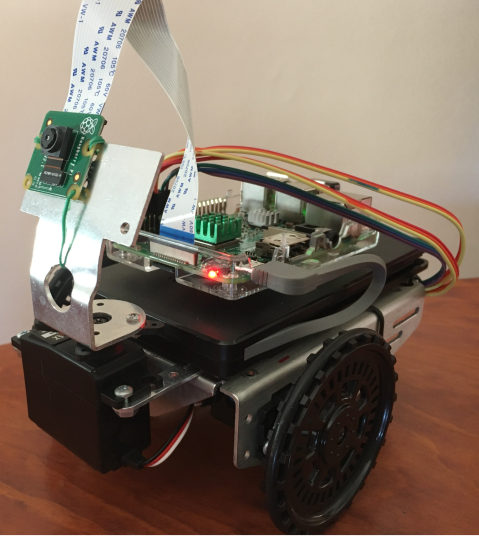
\includegraphics[width=6cm]{figs/cap5/Original.png}
	\end{center}
	\caption{Pibot} 
	\label{fig:pibot}
\end{figure}

Para poder continuar con la investigación de este proyecto, se creó una estructura de metal para que la cámara cambiase su disposición, mirase hacia el suelo y estuviese del derecho para evitar futuros cálculos innecesarios. El diseño hasta ese momento quedó como muestra la Figura \ref{fig:pibotmetal}.


\begin{figure} [h!]
	\begin{center}
		\includegraphics[width=8cm]{figs/cap5/new.png}
	\end{center}
	\caption{Pibot con cámara modificada} 
	\label{fig:pibotmetal}
\end{figure}


De este robot interesa que tiene dos grados de libertad para el movimiento del robot, ya que cuenta con dos ruedas con motores independientes y una rueda loca, lo que le permite desplazarse a lo largo del eje X como girar sobre sí misma. Otro grado de libertad que ha resultado útil para la aplicación de este proyecto es el giro sobre el eje Z del motor sobre el que está montada la cámara y poder aumentar el campo de visión. Así lo muestra la Figura \ref{fig:esquemaDOF}, señalados en rojo.


\begin{figure} [h!]
	\begin{center}
		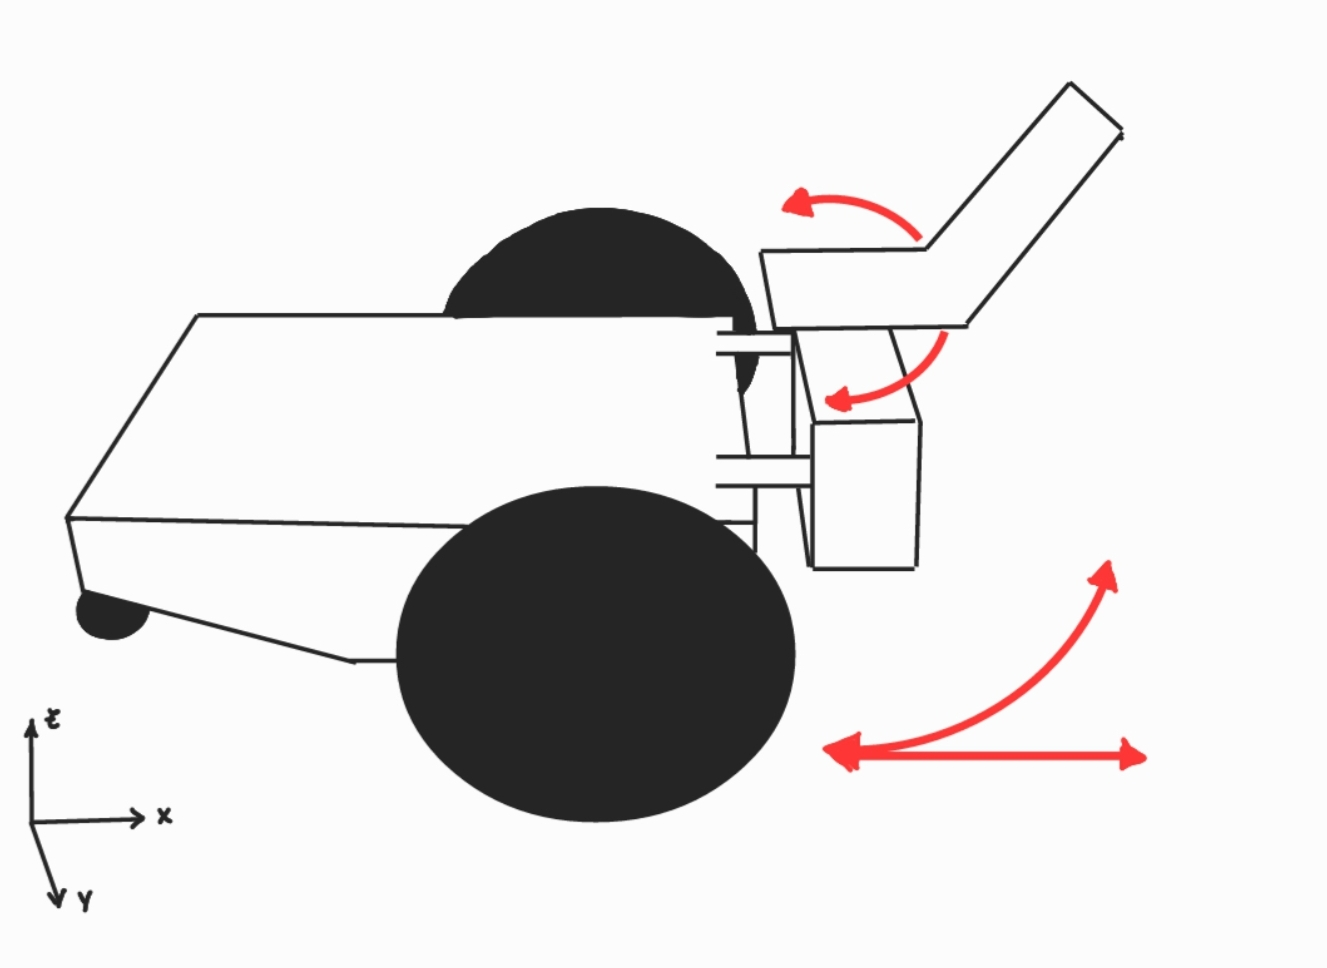
\includegraphics[width=9cm]{figs/cap5/dof.jpg}
	\end{center}
	\caption{Esquema de los grados de libertad de Pibot} 
	\label{fig:esquemaDOF}
\end{figure}


Para poder cumplir con el objetivo principal descrito en el Capítulo 3, es necesario añadir una serie de componentes \textit{hardware} para poder formar el esqueleto completo del robot.

\section{Elección de componentes hardware}

Una vez definida la geometría del robot, es necesario elegir los componentes que más se ajustan para poder confeccionar el esqueleto del robot. Para ellos se ha creado un esquema (Figura \ref{fig:fritzzing}) que muestra todos los componentes necesarios y sus conexiones. A continuación, se van a explicar cada uno de los componentes \textit{hardware} elegidos.  

\begin{figure} [h!]
	\begin{center}
		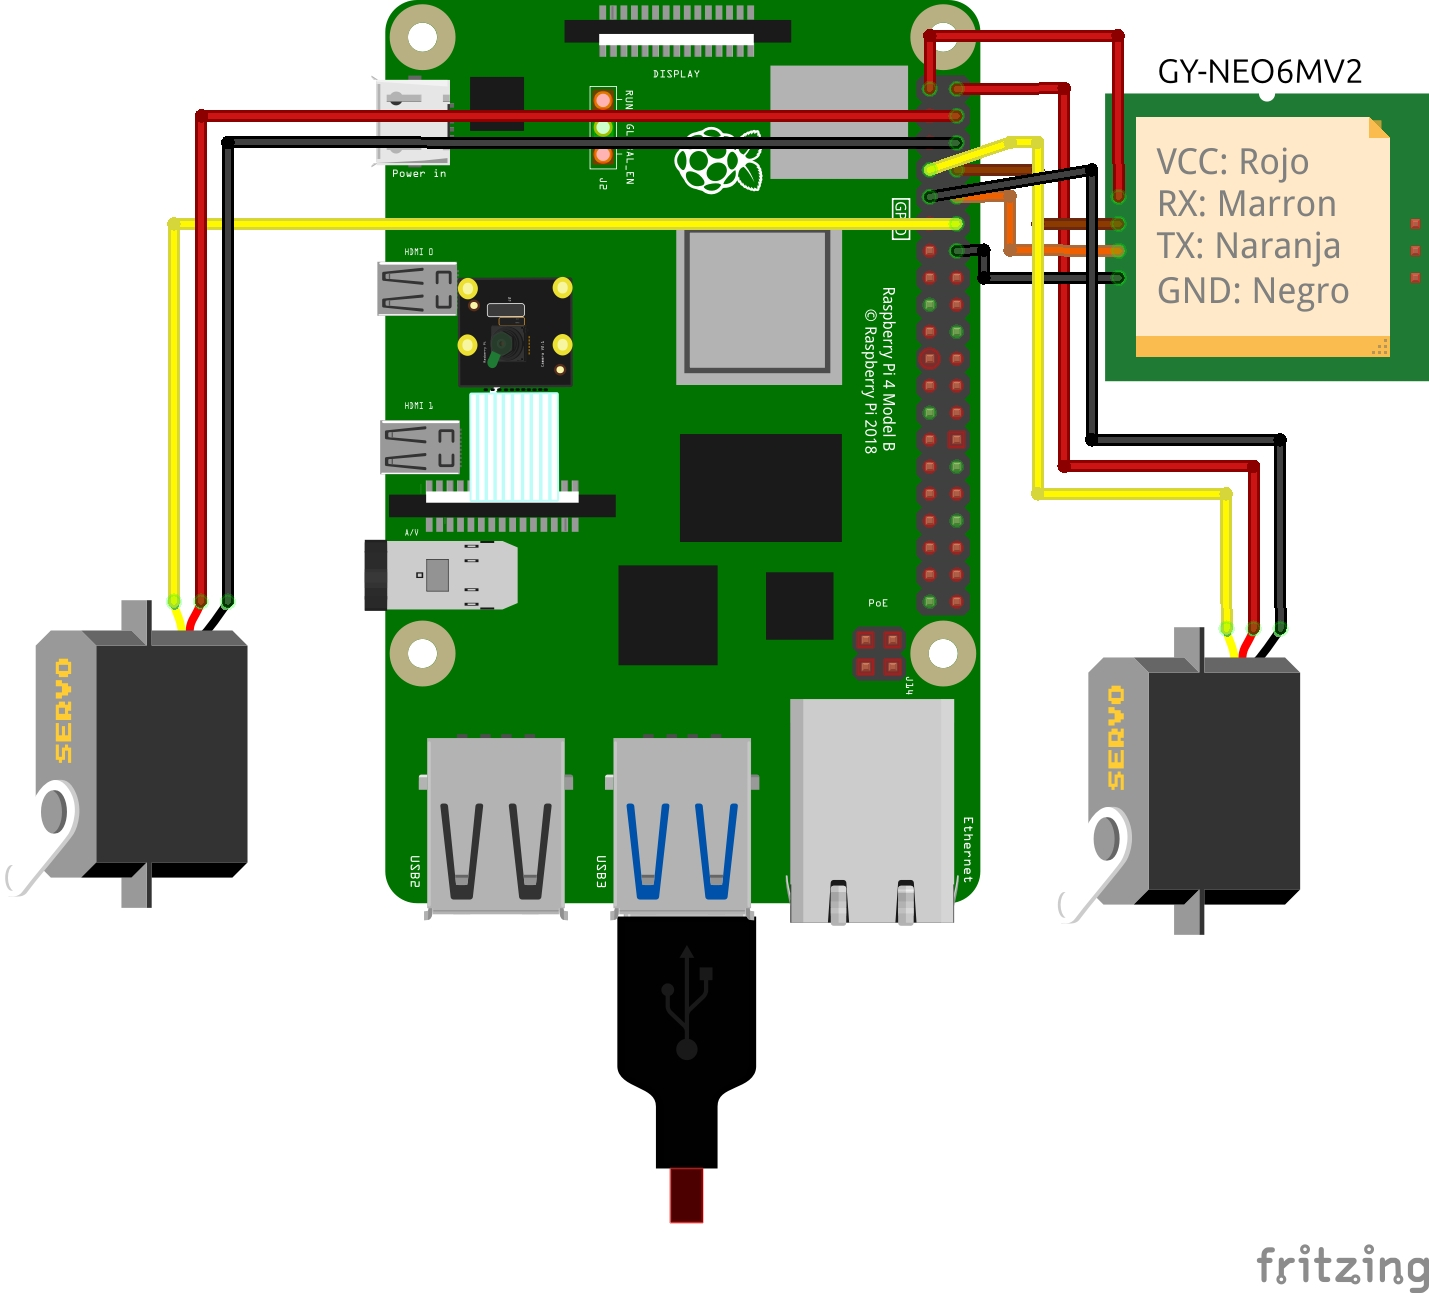
\includegraphics[width=9cm]{figs/cap5/modelocompleto_bb.jpg}
	\end{center}
	\caption{Esquema de conexiones del robot} 
	\label{fig:fritzzing}
\end{figure}


\subsection{Raspberry Pi 4}

Es muy usado en robótica, ordenador a bordo,....



\subsection{Servomotores Parallax}
La fuerza, la utilidad que hacen,...


\subsection{Ruedas ActivityBot}
La fuerza, la utilidad que hacen,...

\subsection{Rueda Loca}
La fuerza, la utilidad que hacen,...

\subsection{Raspberry Pi Cámara}

Calidad de la imagen, parámetros intrínsecos teóricos,... 

\subsection{GPS NEO 6M}
Explicar el módulo GPS .... pruebas, alcance... tarda en coger señal, la luz azul...

\subsection{Google Coral USB}

Utilidades, el nivel de cómputo que llega,... inferencias por segundo,tipo de modelos compatible...

\subsection{Powerbank}
 
 Todo el día encendida y ejecutando, aguanta perfectamente... \\
 
  
  
 Distribuir los componentes (foto de fritzing): motores, sensores, cámaras (fotos mías)
 
 
 Explicar todos los componentes usados: 
 
 Si se incluyen imágenes que sean distintas a las del apartado de plataformas de desarrollo o no incluirlas. 
 
 Fotos hechas por mí 
 
 Uso las características que he aprovechado del capítulo 4 
 
 
\section{Bocetos}

La realización de bocetos es una etapa fundamental en el proceso de diseño que se realiza antes de iniciar el modelado en 3D, ya que su propósito es obtener una visión clara de la estructura y disposición de los componentes que conforman el robot. Una vez que se ha definido el esqueleto completo que este necesitará, es el momento de crear una serie de bocetos (Figura \ref{fig:bocetos}) que permitirán afinar los detalles antes de realizar el diseño en 3D.

\begin{figure}[ht!]
	\centering
	\begin{minipage}{0.4\linewidth}
		\centering
		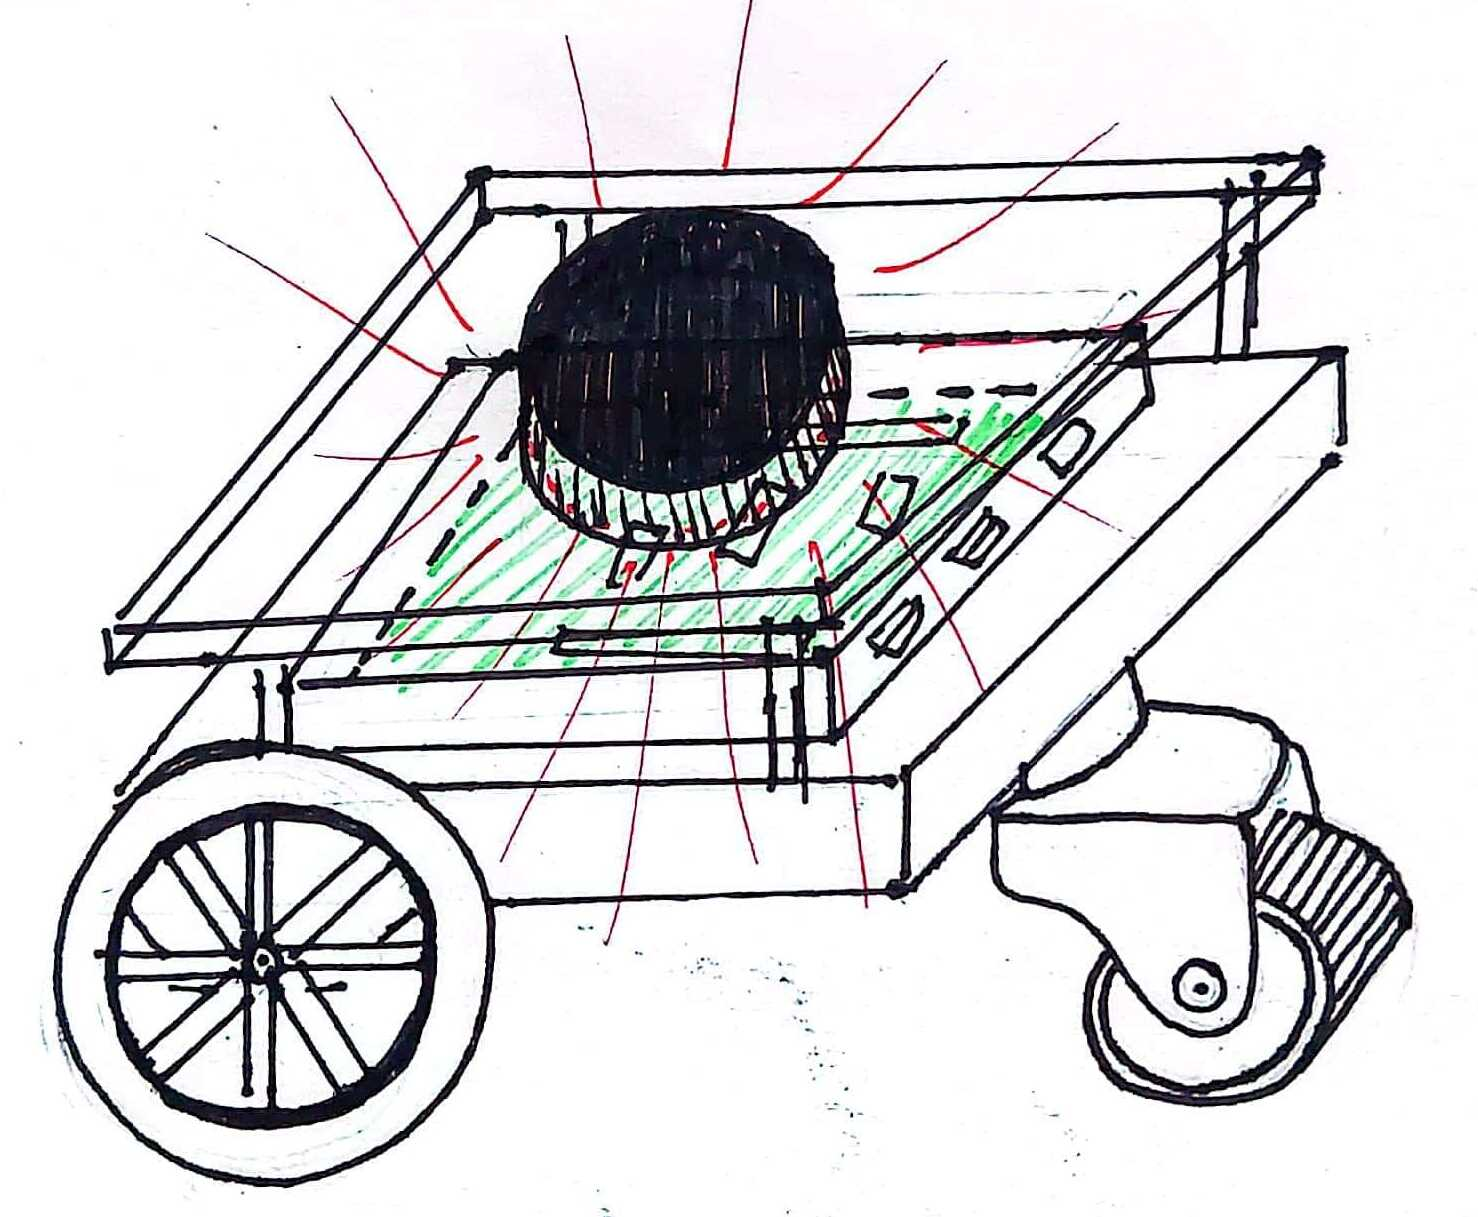
\includegraphics[width=\linewidth]{figs/cap5/prototipo_laser.jpeg}
	\end{minipage}
	\hspace{2cm}
	\begin{minipage}{0.4\linewidth}
		\centering
		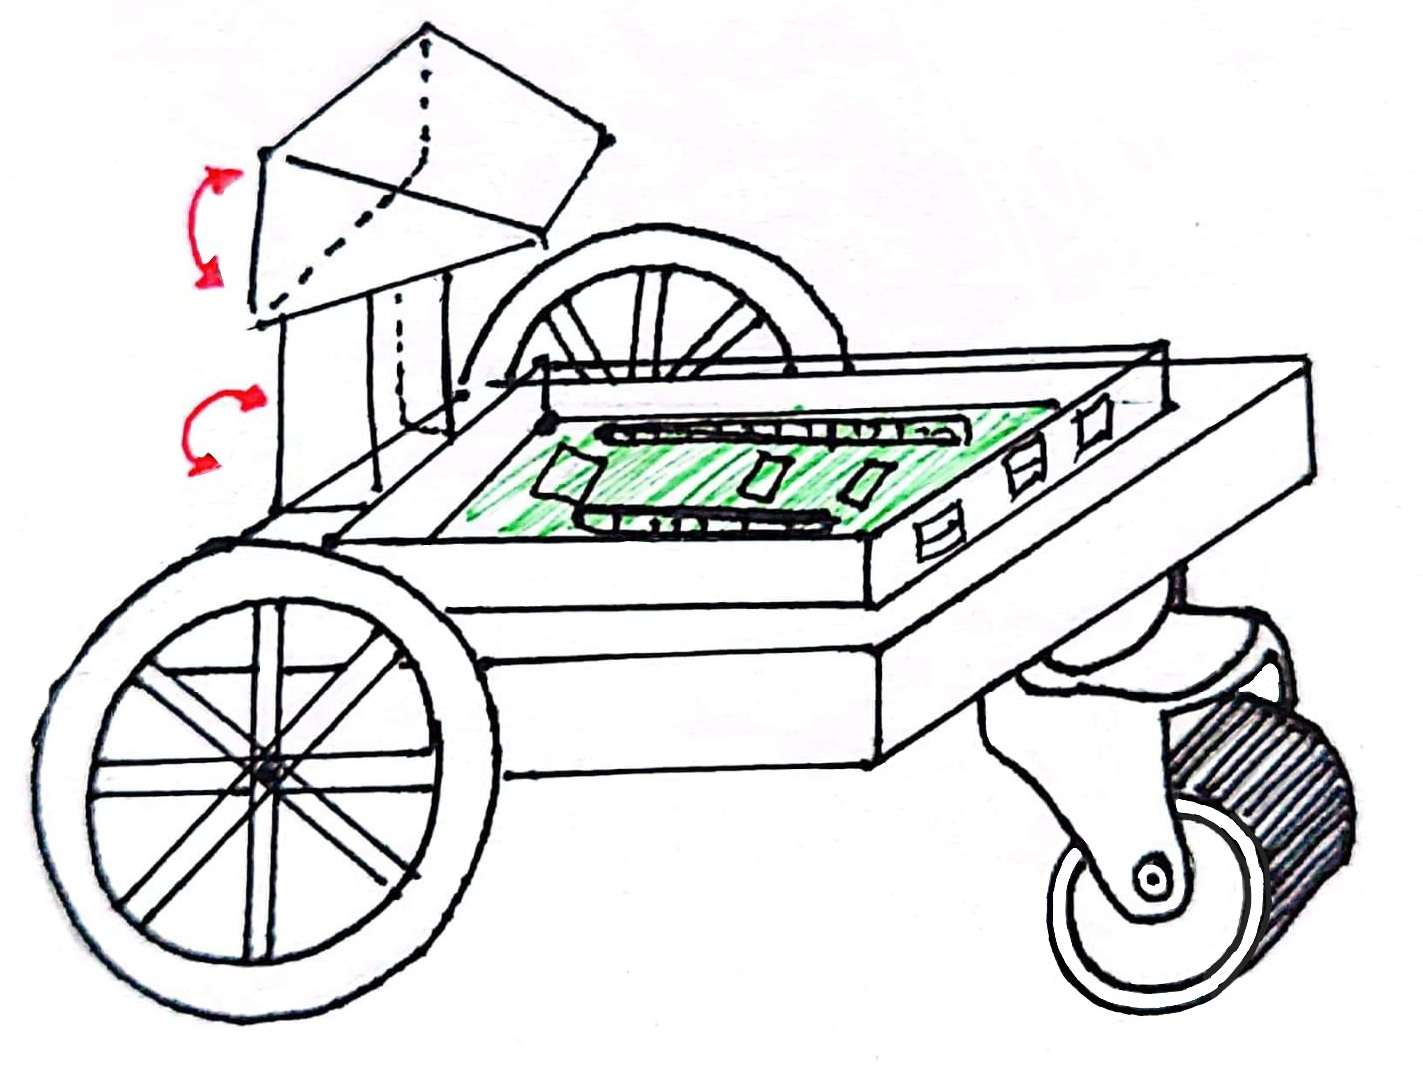
\includegraphics[width=\linewidth]{figs/cap5/prototipo_sin_laser.jpeg}
	\end{minipage}
	\hspace{2cm}
	\begin{minipage}{0.5\linewidth}
		\centering
		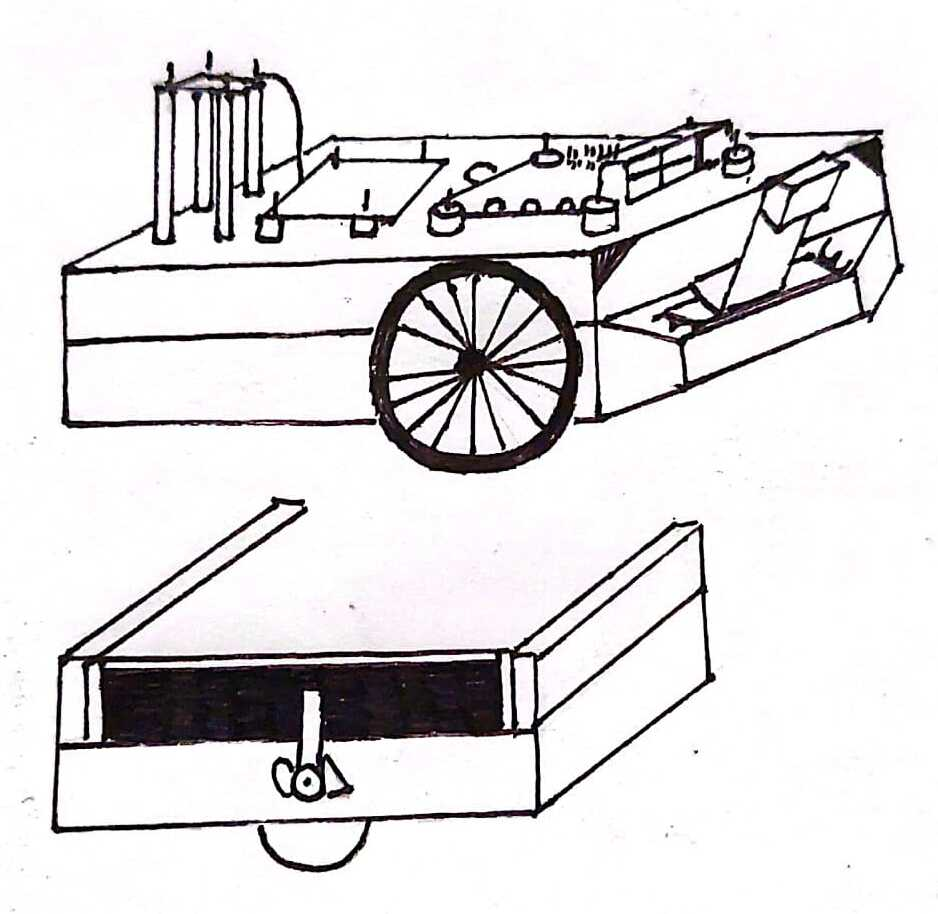
\includegraphics[width=\linewidth]{figs/cap5/boceto_papel.jpeg}
	\end{minipage}
	\caption{Bocetos creados a mano}
	\label{fig:bocetos}
\end{figure}

Antes de realizar el diseño \acs{CAD} de las piezas, se creó una maqueta a tamaño real (Figuras \ref{fig:maqueta1} y \ref{fig:maqueta2}) para poder tener una idea de cómo sería la aplicación final y así intentar no malgastar material de impresión. 

\begin{figure}[ht!]
	\centering
	\begin{minipage}{0.5\linewidth}
		\centering
		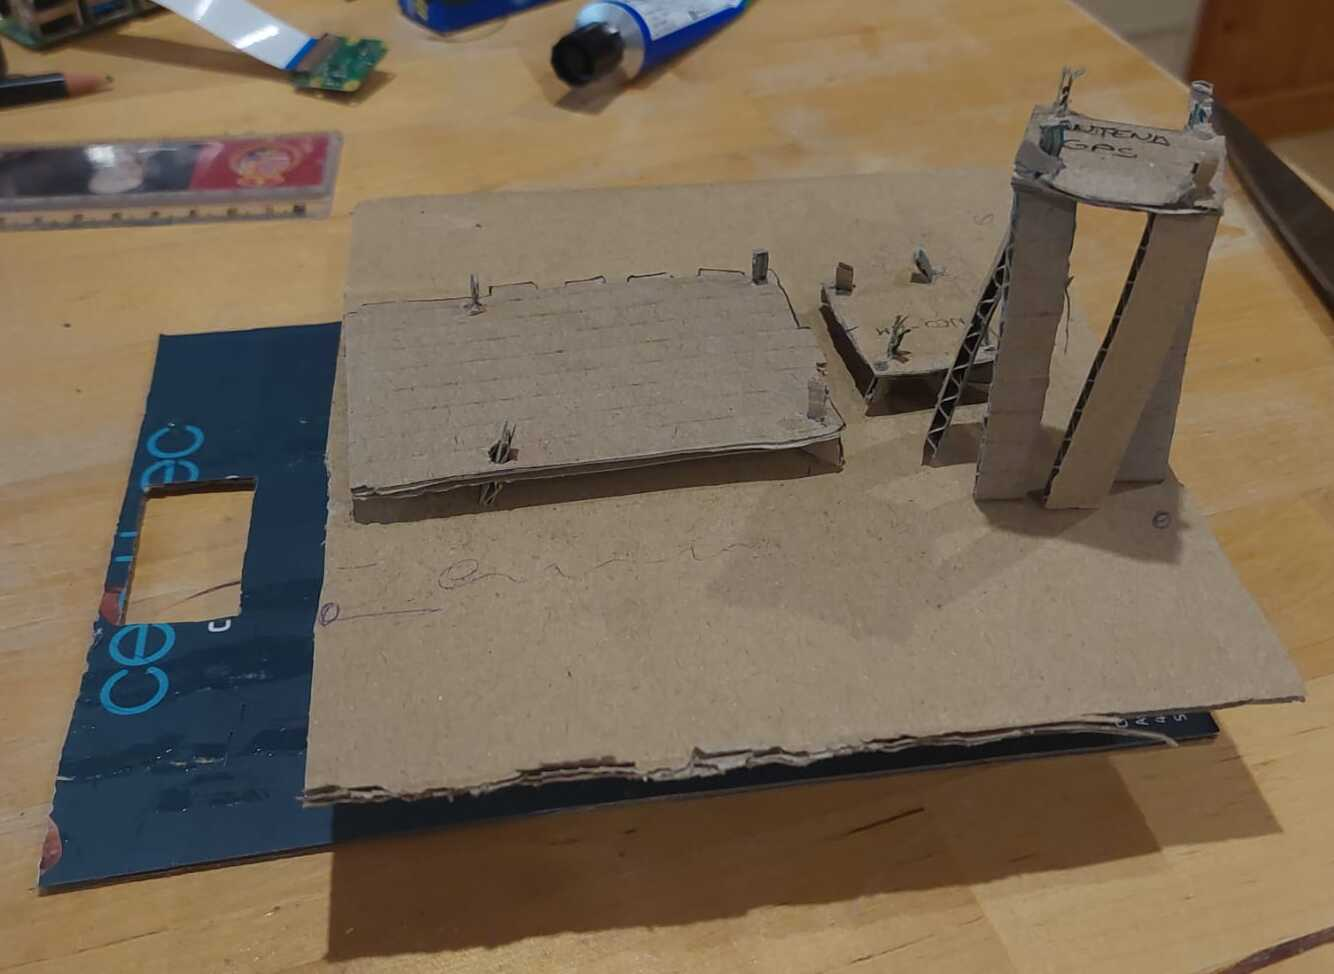
\includegraphics[width=\linewidth]{figs/cap5/boceto_carton1.jpeg}
		\caption*{\centering}
	\end{minipage}
	\hspace{1cm}
	\begin{minipage}{0.4\linewidth}
		\centering
		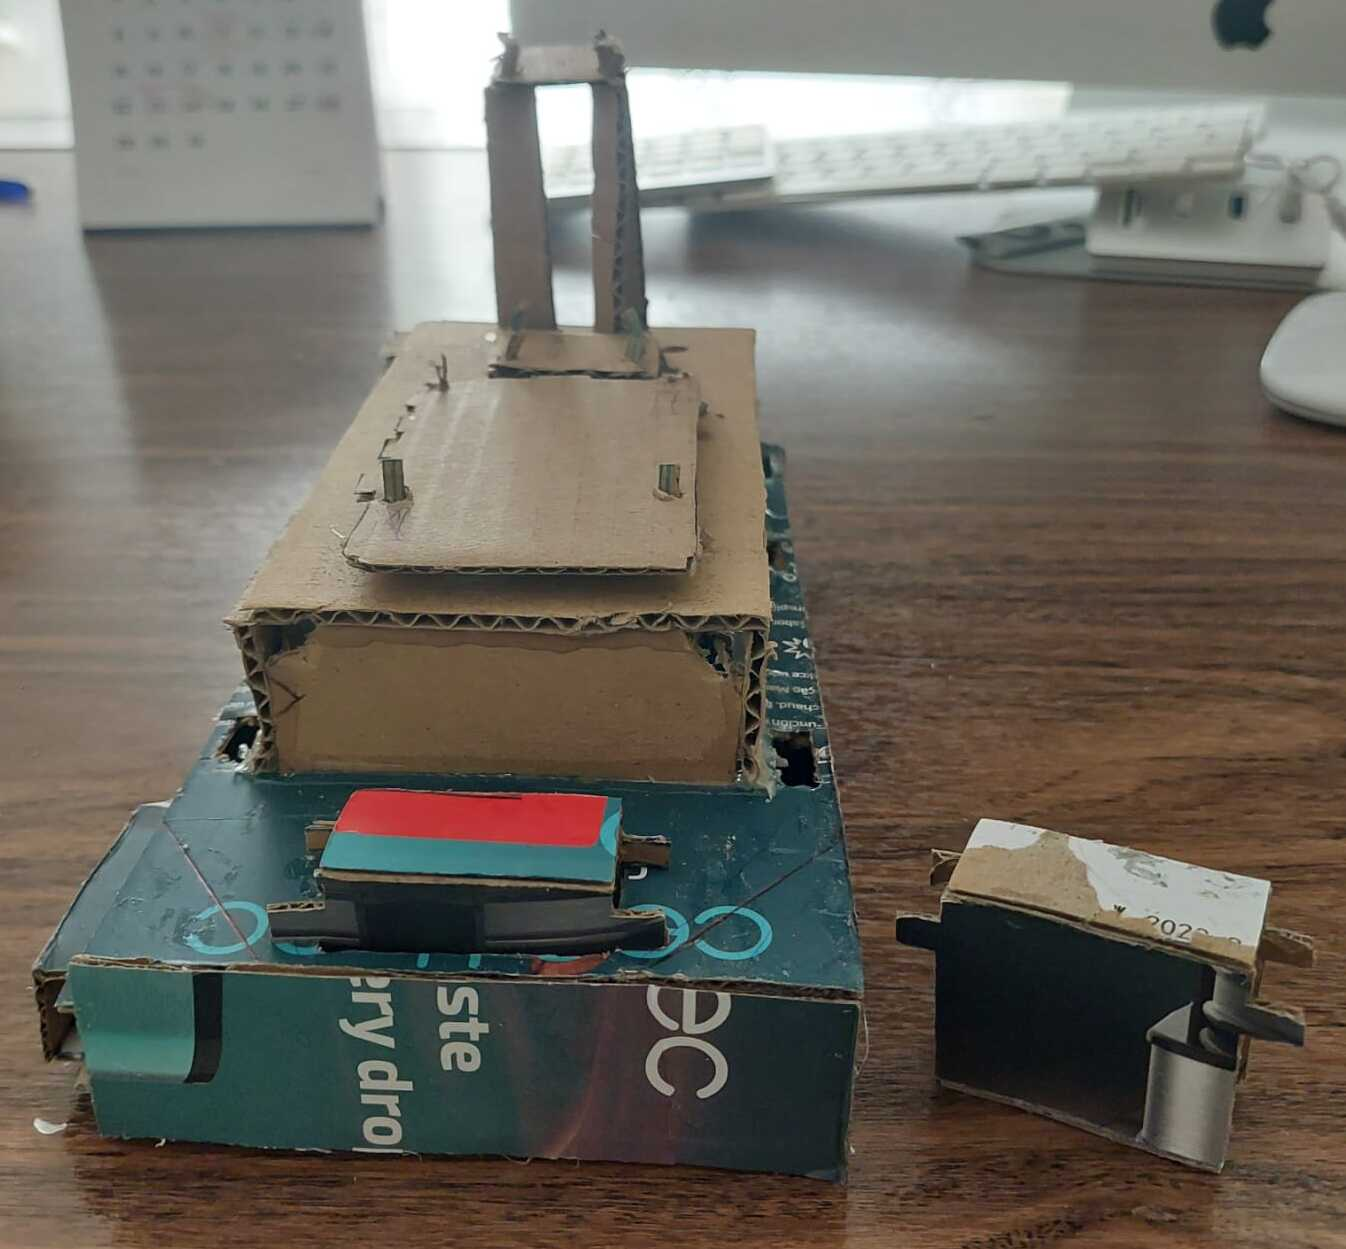
\includegraphics[width=\linewidth]{figs/cap5/boceto_carton2.jpeg}
		\caption*{\centering}
	\end{minipage}
	\hspace{2cm}
	\begin{minipage}{0.4\linewidth}
		\centering
		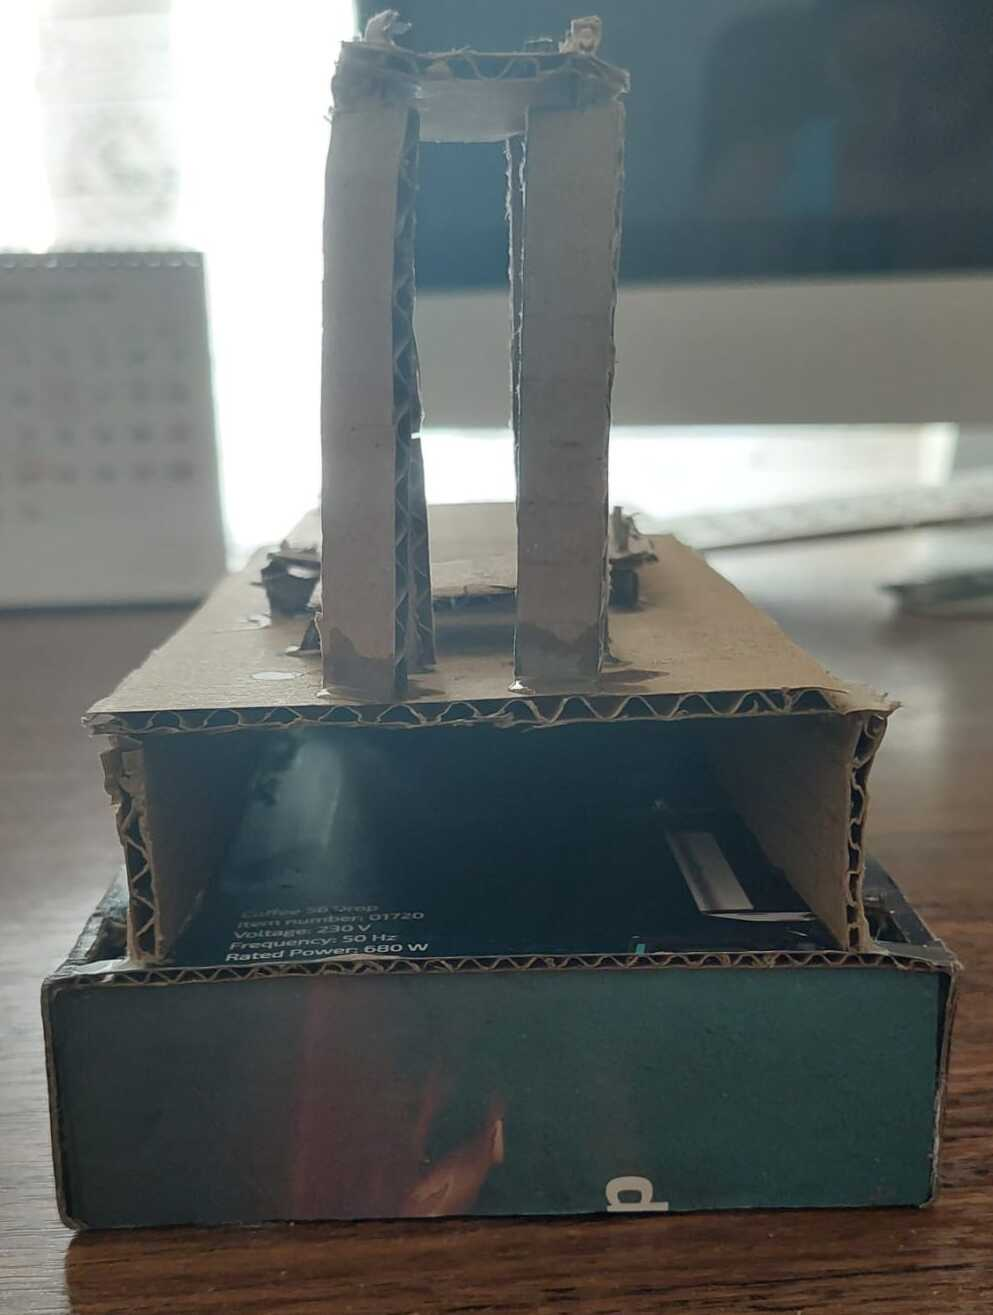
\includegraphics[width=\linewidth]{figs/cap5/boceto_carton3.jpeg}
		\caption*{\centering}
	\end{minipage}
	\caption{Maqueta en proceso}
	\label{fig:maqueta1}
\end{figure}

\begin{figure}[ht!]
	\centering
	\begin{minipage}{0.44\linewidth}
		\centering
		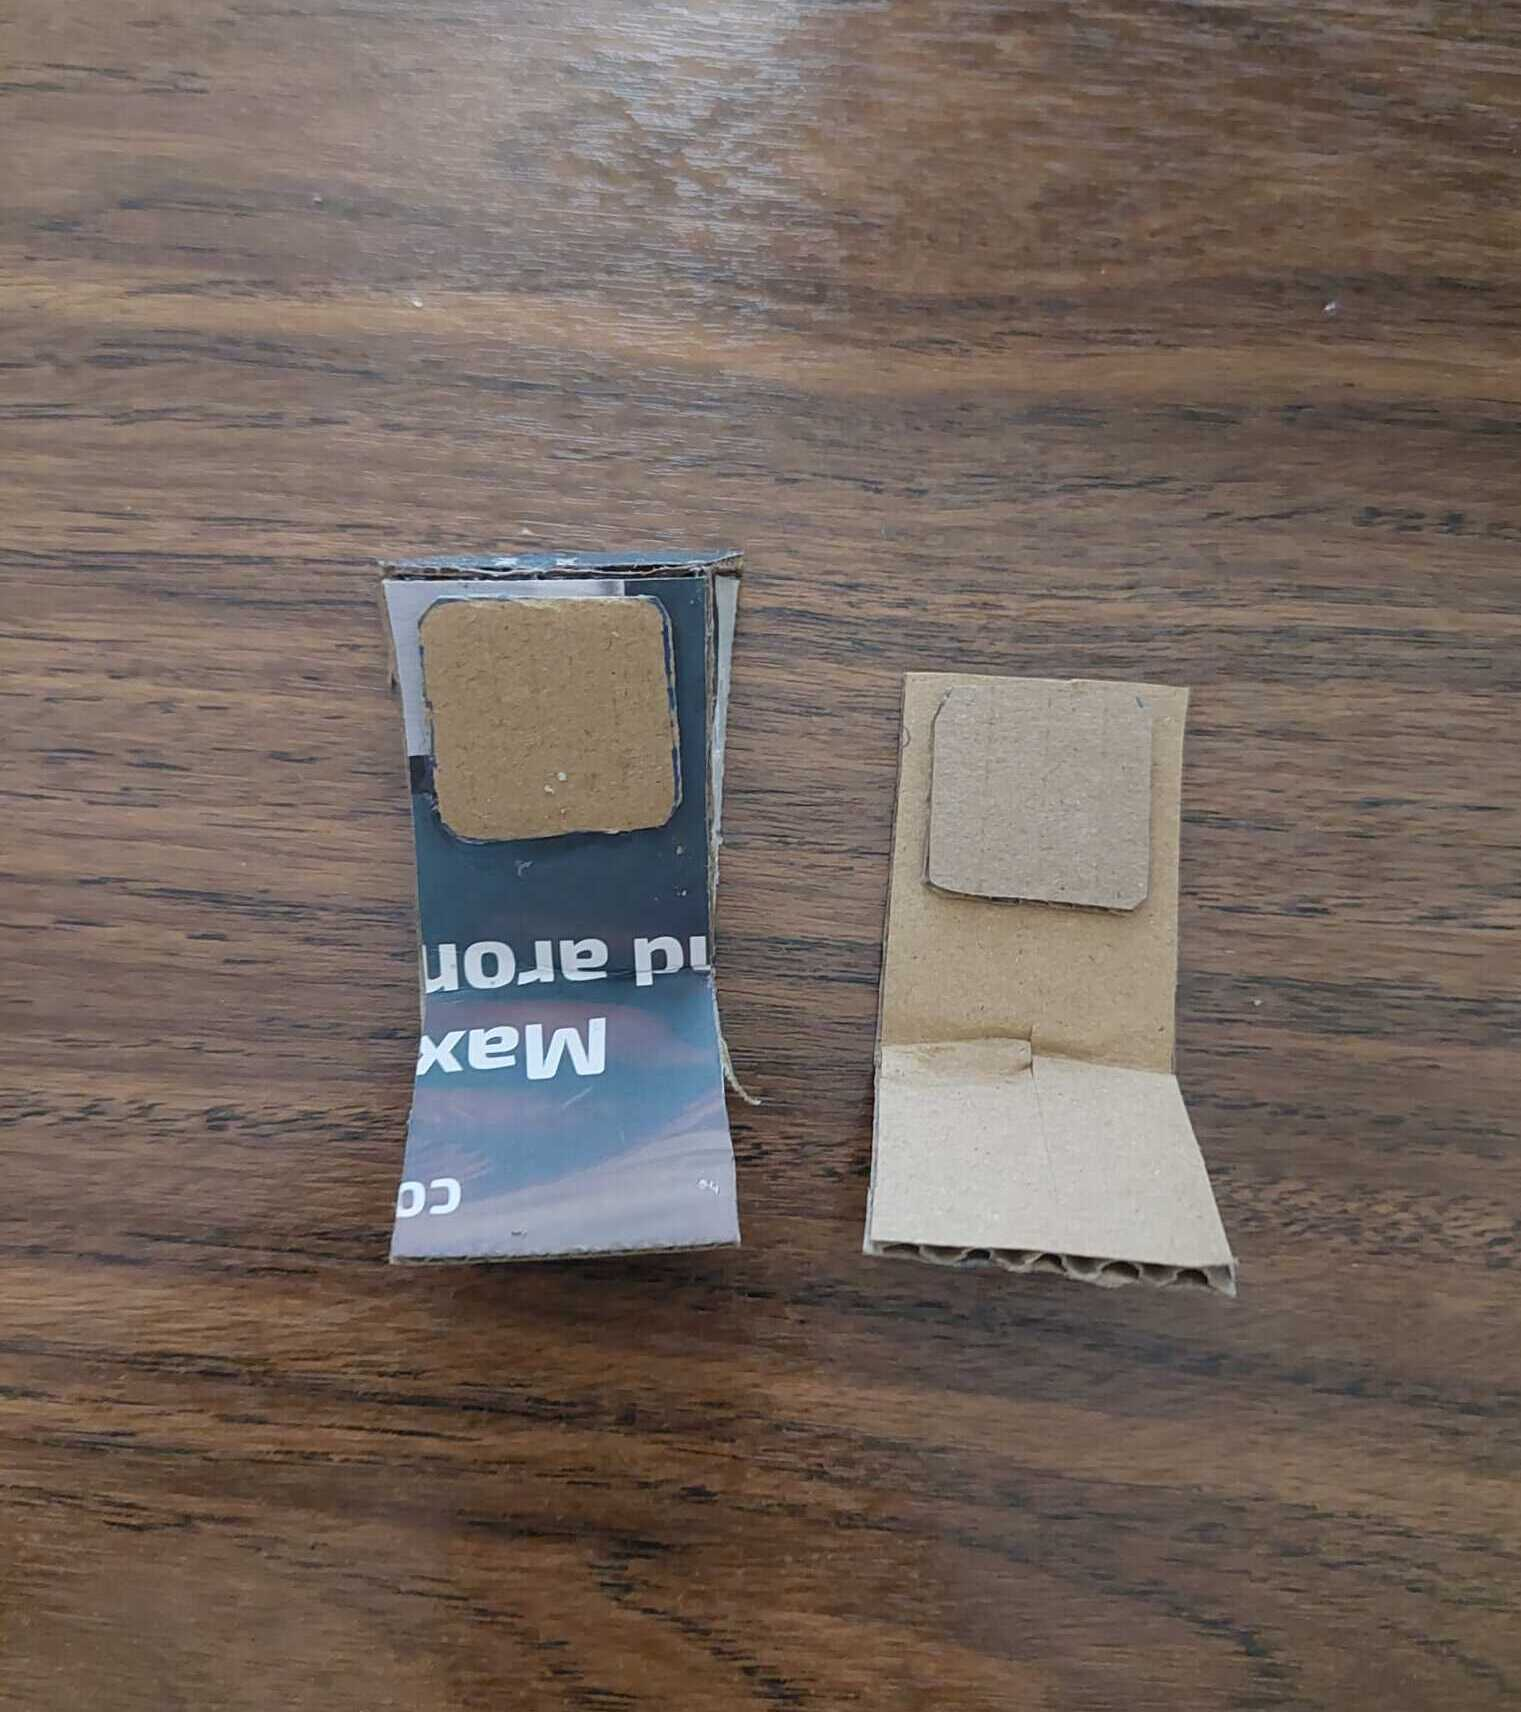
\includegraphics[width=\linewidth]{figs/cap5/boceto_carton4.jpeg}
		\caption*{\centering}
	\end{minipage}
	\hspace{2cm}
	\begin{minipage}{0.4\linewidth}
		\centering
		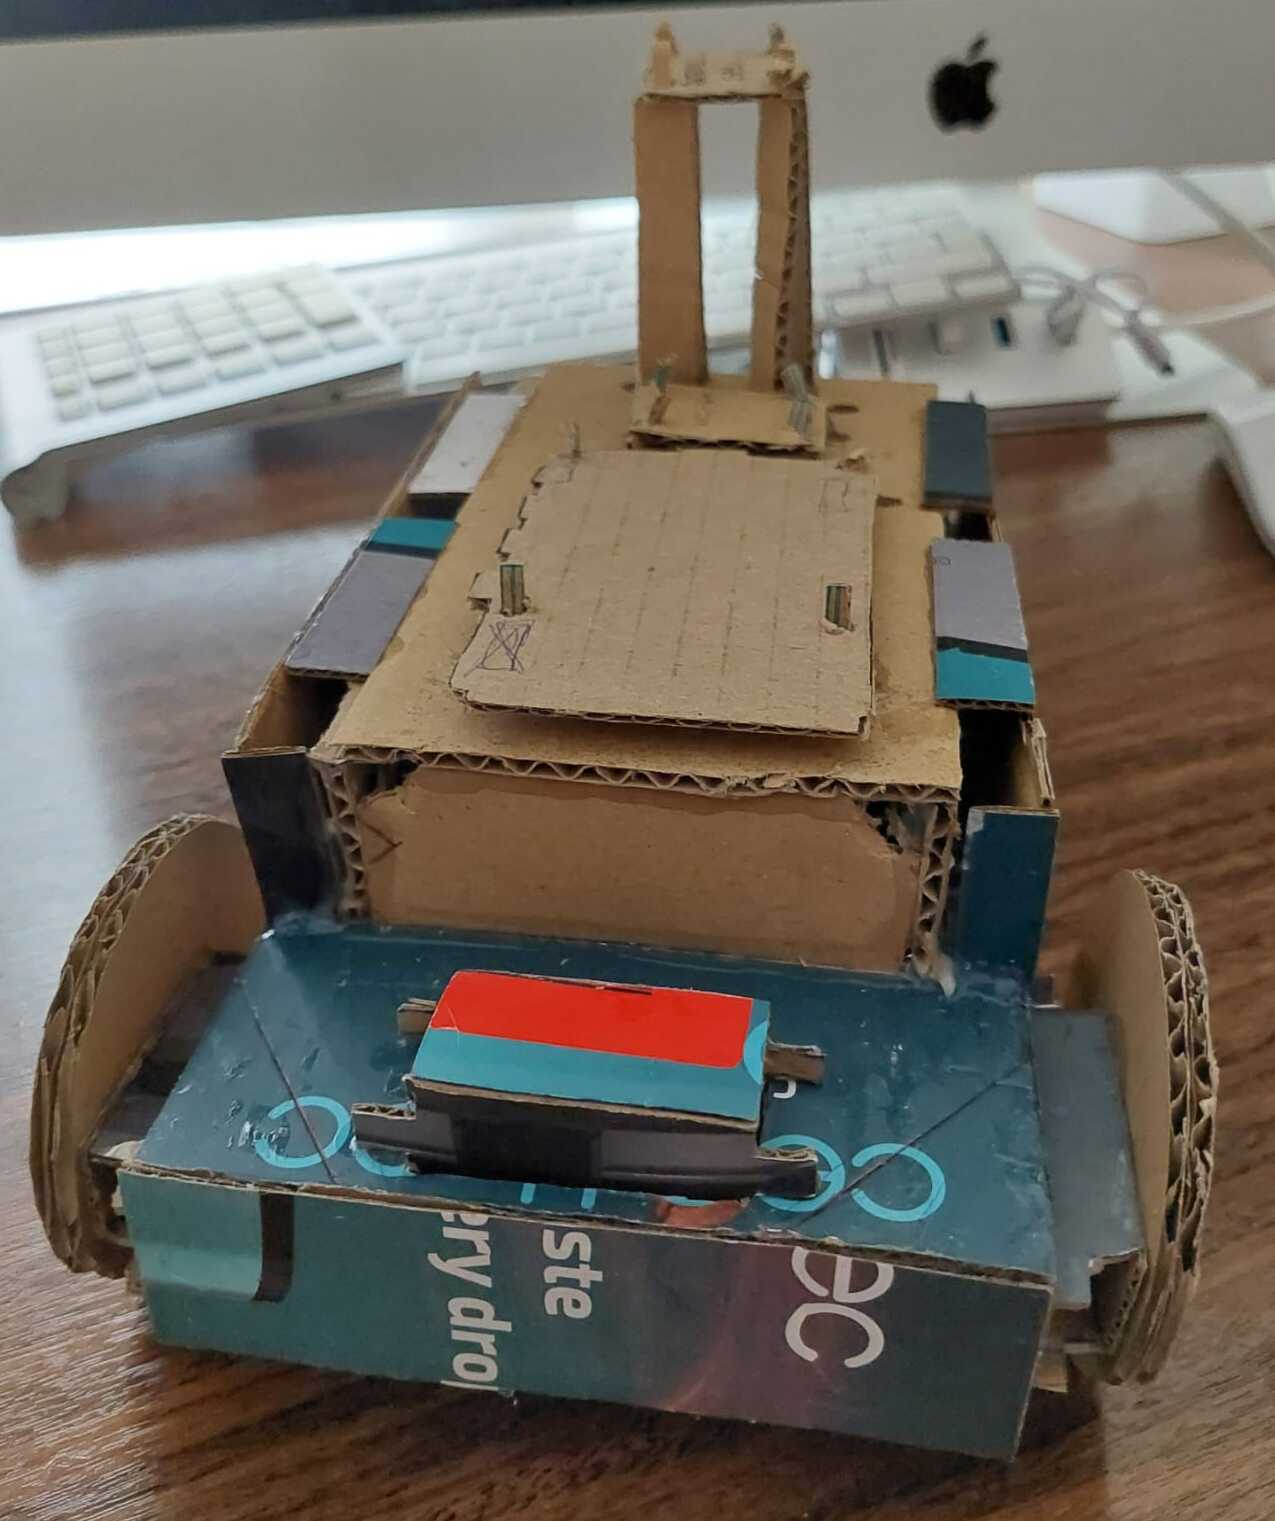
\includegraphics[width=\linewidth]{figs/cap5/boceto_carton5.jpeg}
		\caption*{\centering}
	\end{minipage}
	\hspace{2cm}
	\begin{minipage}{0.45\linewidth}
		\centering
		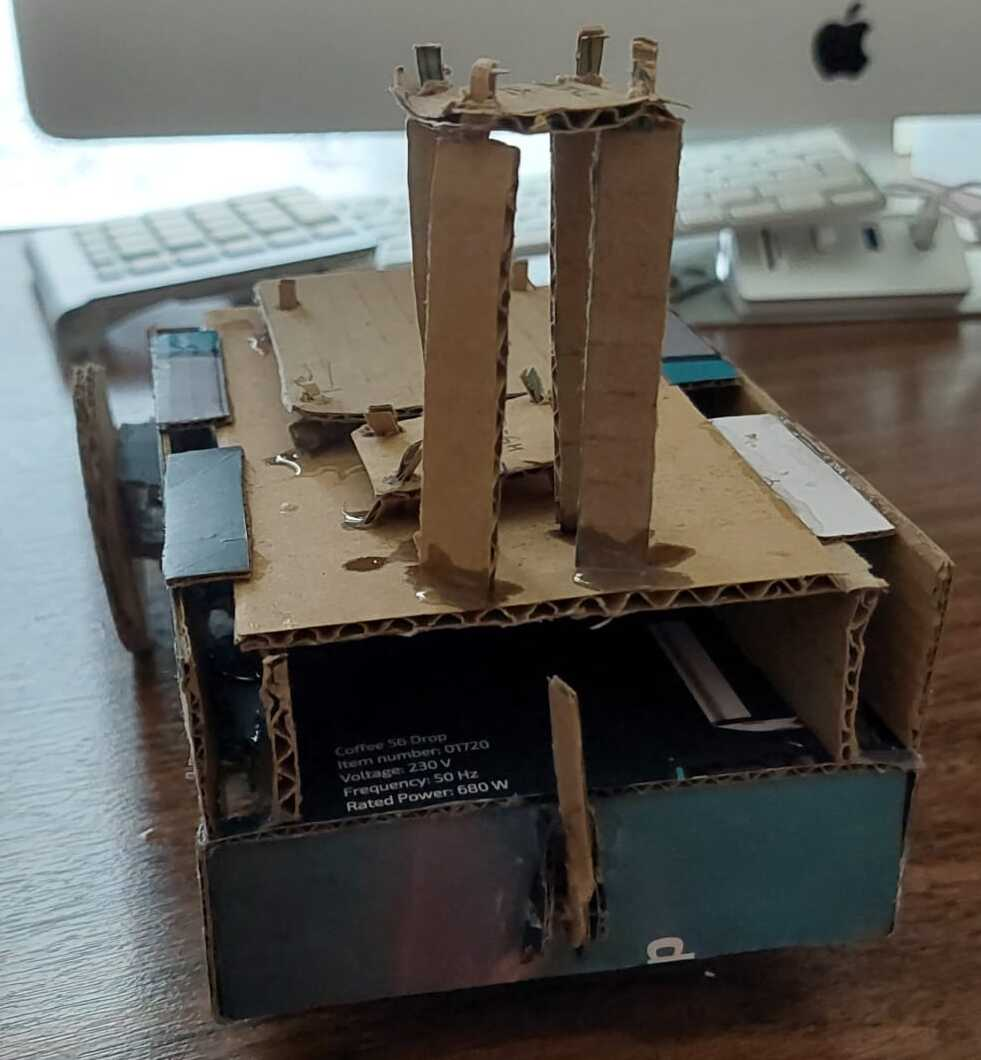
\includegraphics[width=\linewidth]{figs/cap5/boceto_carton6.jpeg}
		\caption*{\centering}
	\end{minipage}
	\hspace{2cm}
	\begin{minipage}{0.4\linewidth}
		\centering
		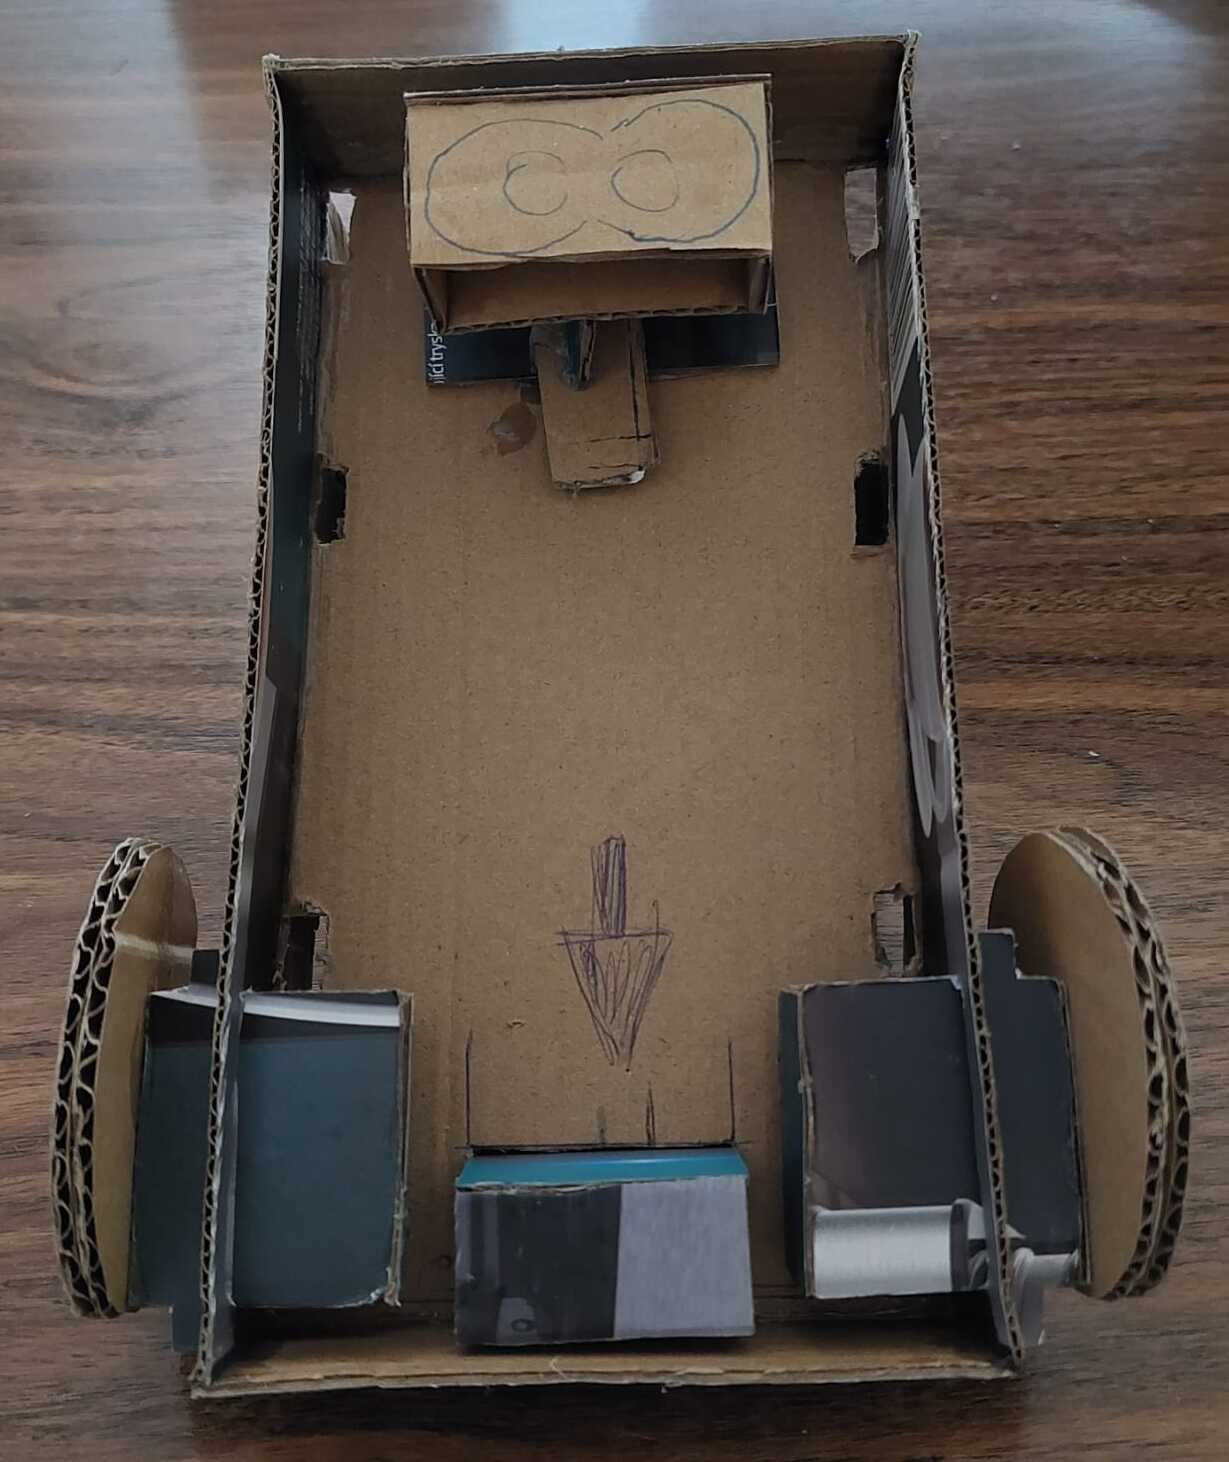
\includegraphics[width=\linewidth]{figs/cap5/boceto_carton7.jpeg}
		\caption*{\centering}
	\end{minipage}
	\caption{Maqueta final}
	\label{fig:maqueta2}
\end{figure}

\section{Diseño CAD}

Para hacer el diseño \acs{CAD} y la maqueta explicada en el apartado anterior, se crearon unos planos a mano (Figura \ref{fig:planos}) de las diferentes piezas que estarían involucradas en el diseño. Estas medidas son precisas gracias al uso del calibre (Figura \ref{fig:calibre}).


\begin{figure}[ht!]
	\centering
	\begin{minipage}{0.45\linewidth}
		\centering
		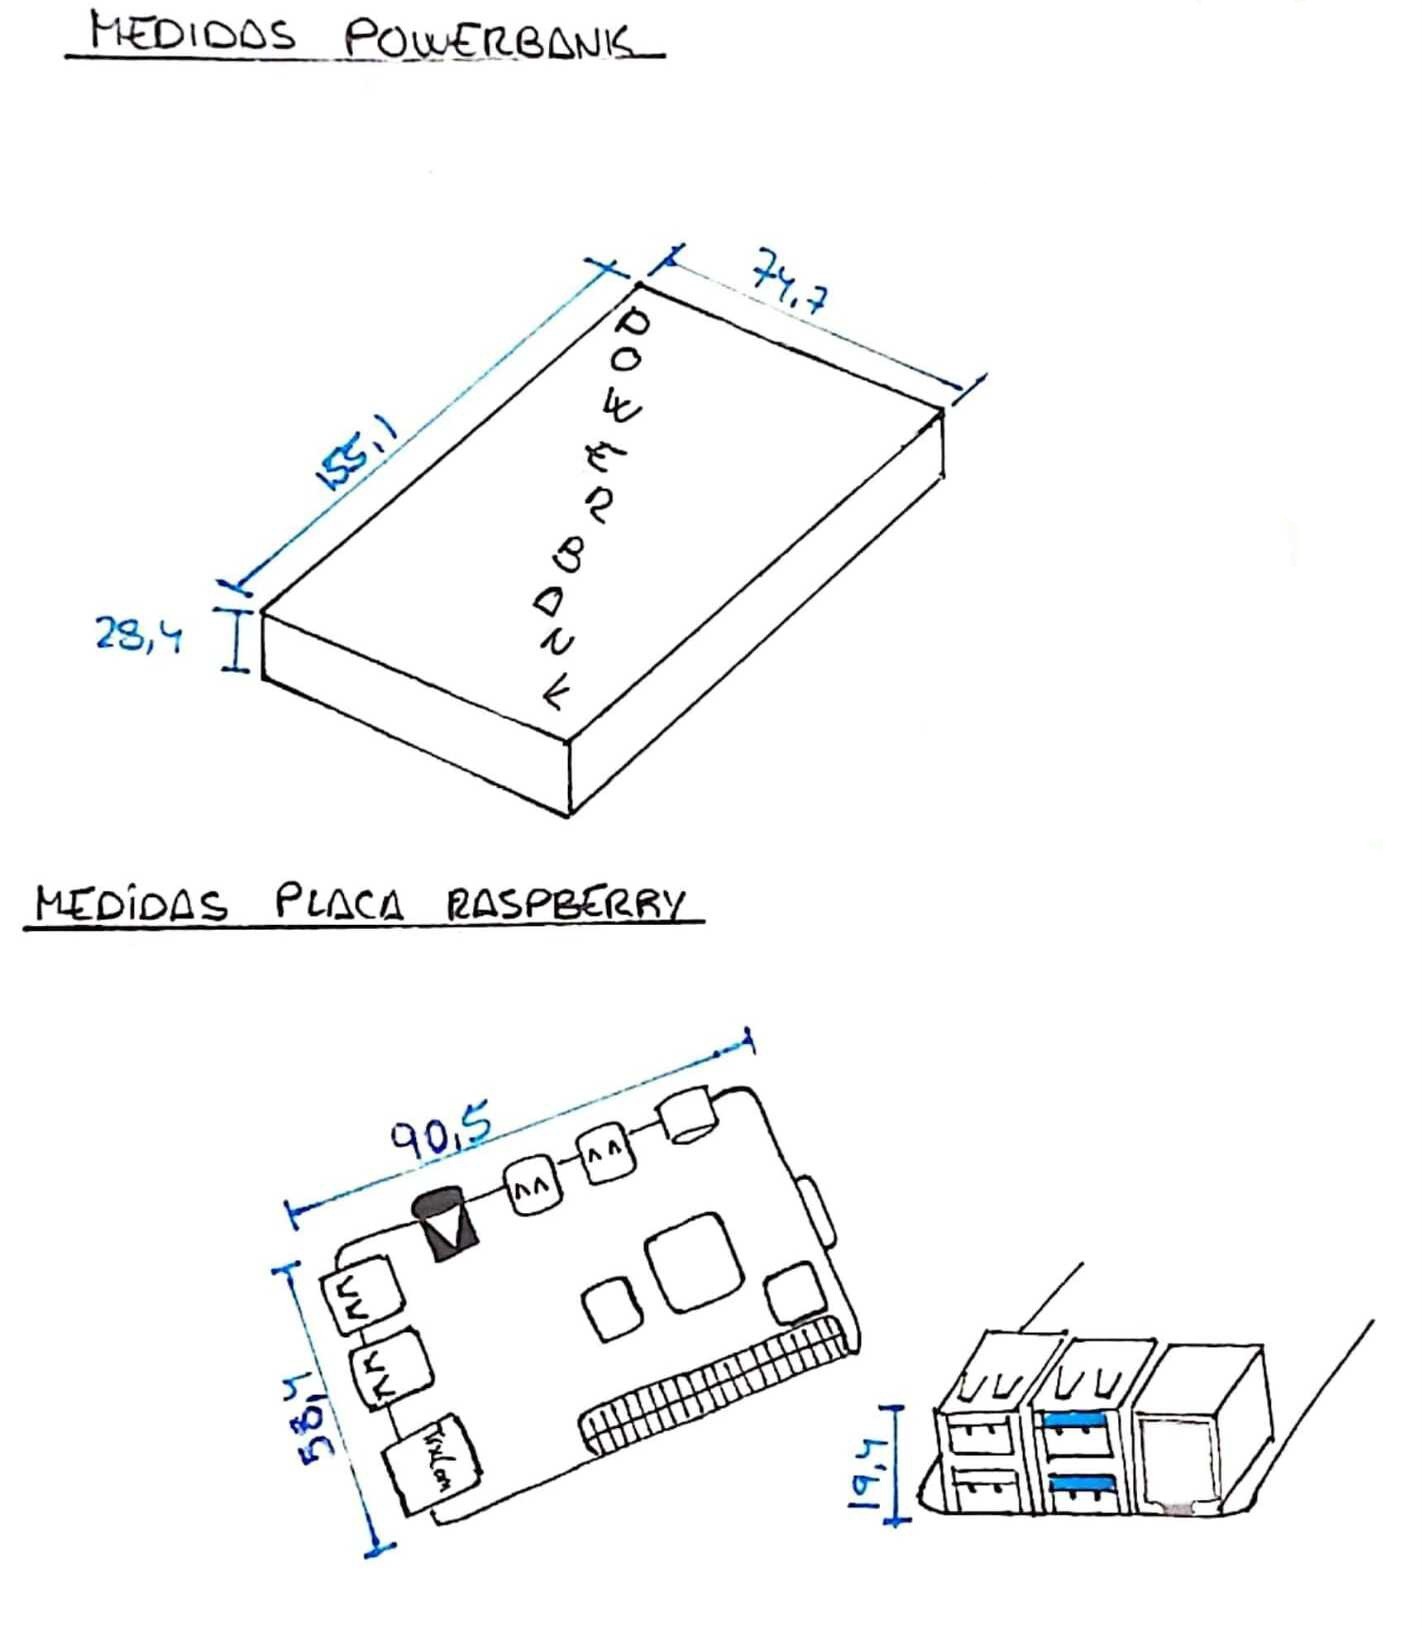
\includegraphics[width=\linewidth]{figs/cap5/planos1.jpeg}
		\caption*{\centering}
	\end{minipage}
	\hspace{1cm}
	\begin{minipage}{0.45\linewidth}
		\centering
		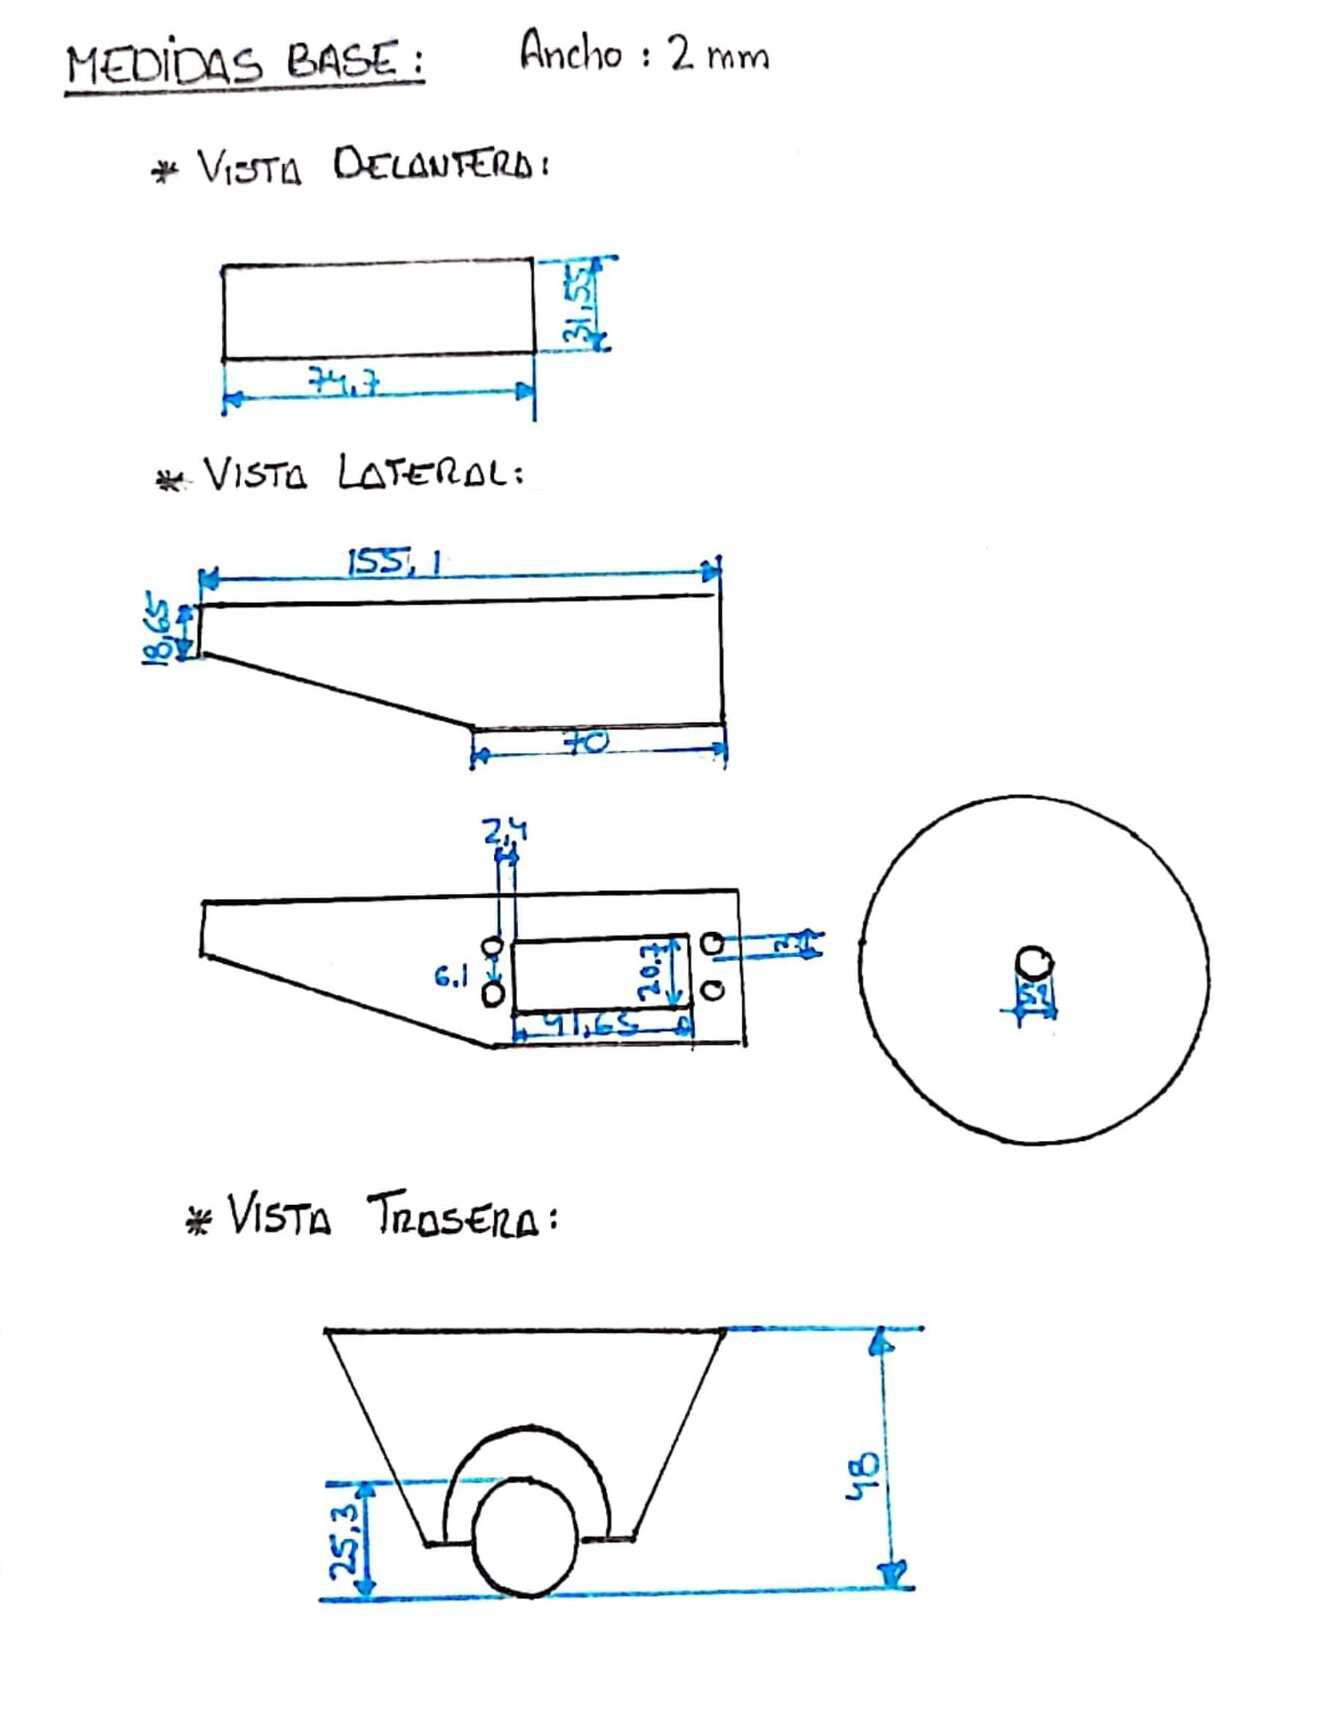
\includegraphics[width=\linewidth]{figs/cap5/planos2.jpeg}
		\caption*{\centering}
	\end{minipage}
	\hspace{1cm}
	\begin{minipage}{0.45\linewidth}
		\centering
		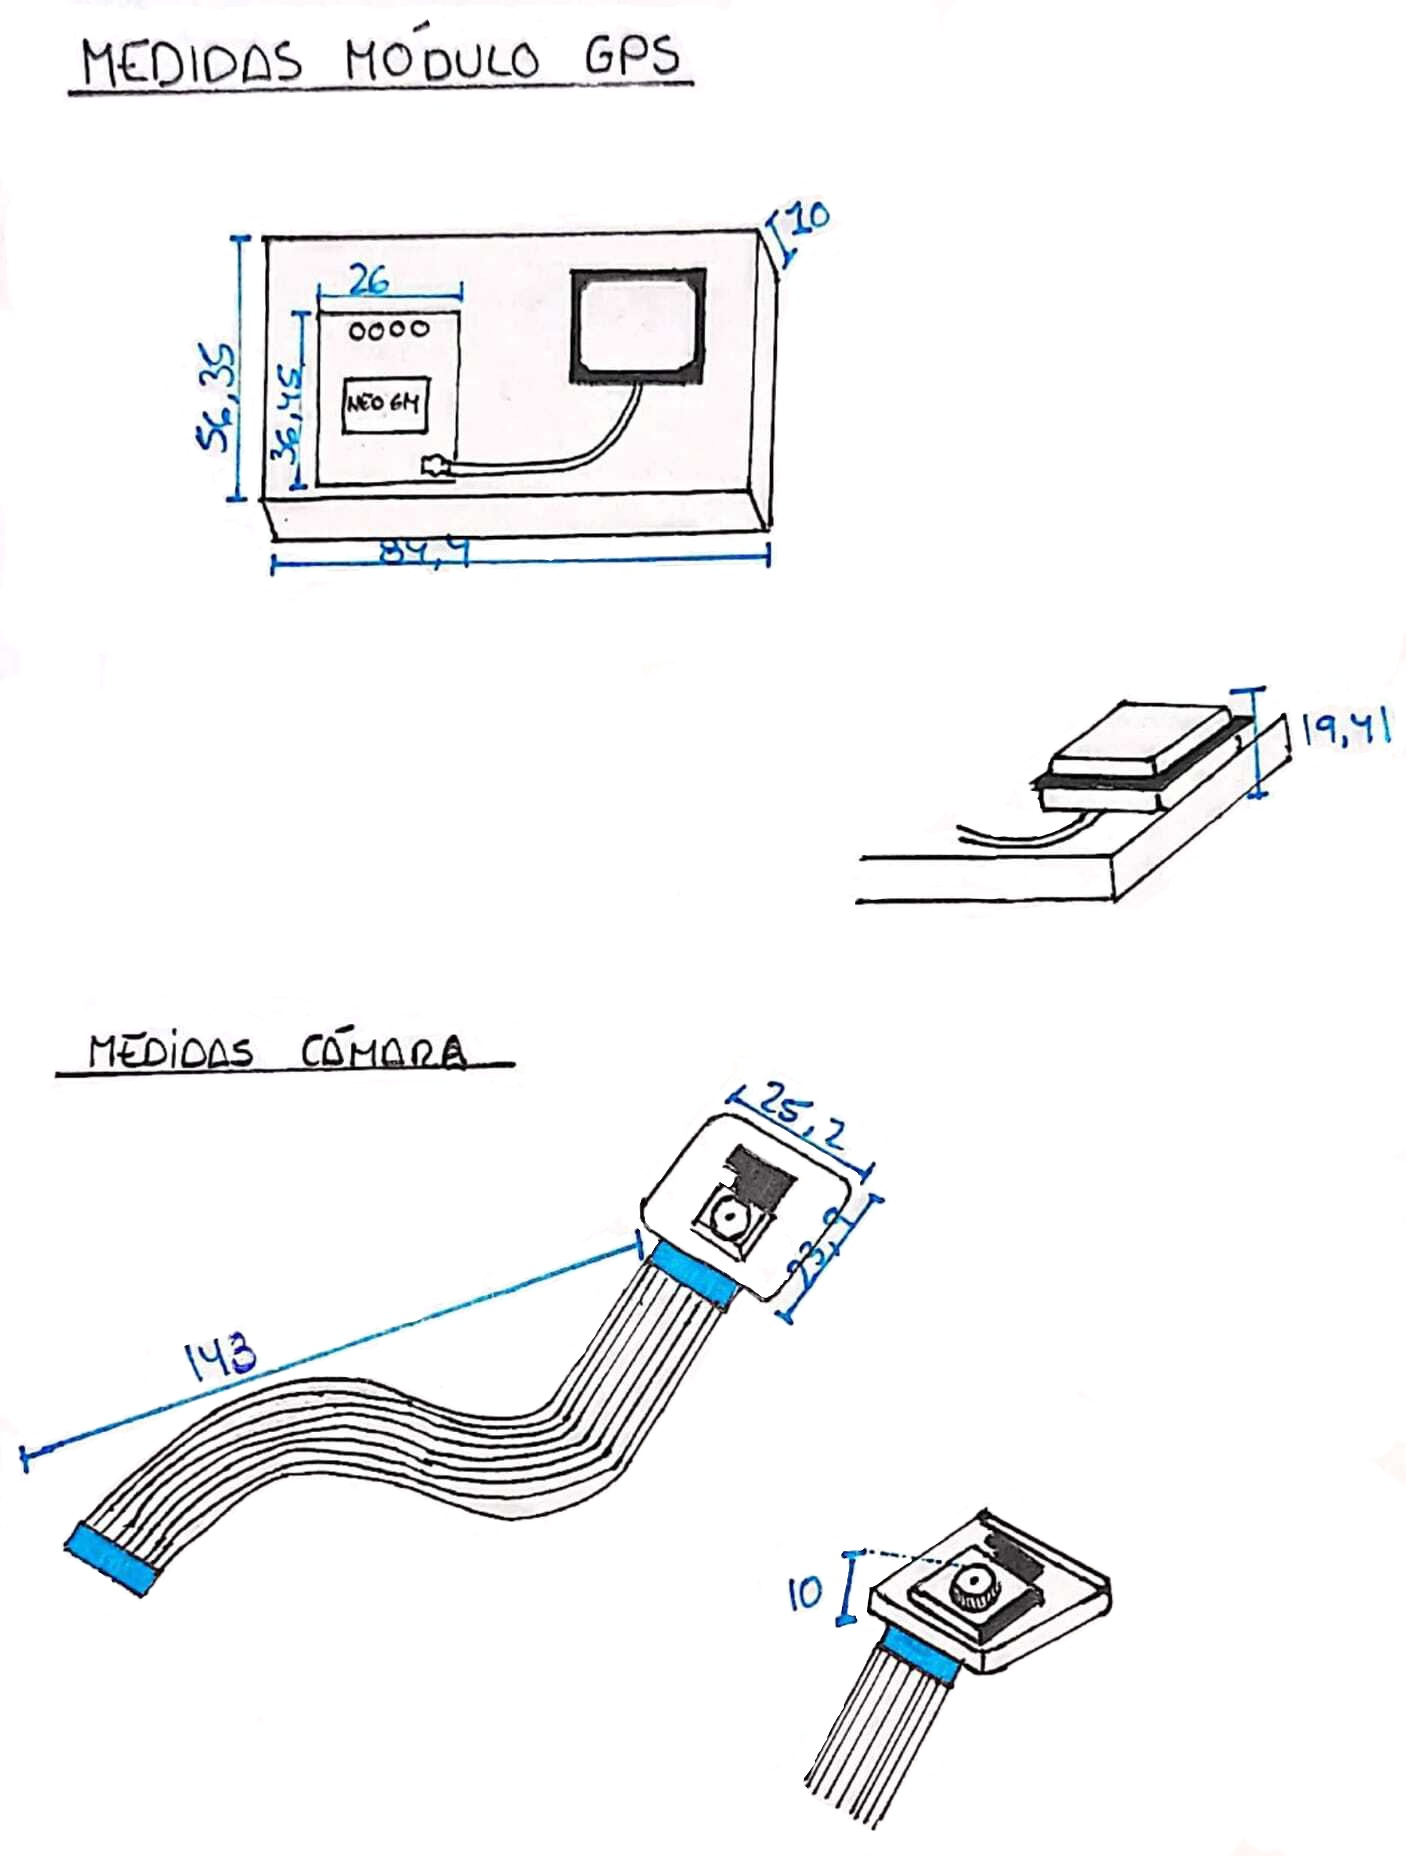
\includegraphics[width=\linewidth]{figs/cap5/planos3.jpeg}
		\caption*{\centering}
	\end{minipage}
	\hspace{1cm}
	\begin{minipage}{0.45\linewidth}
		\centering
		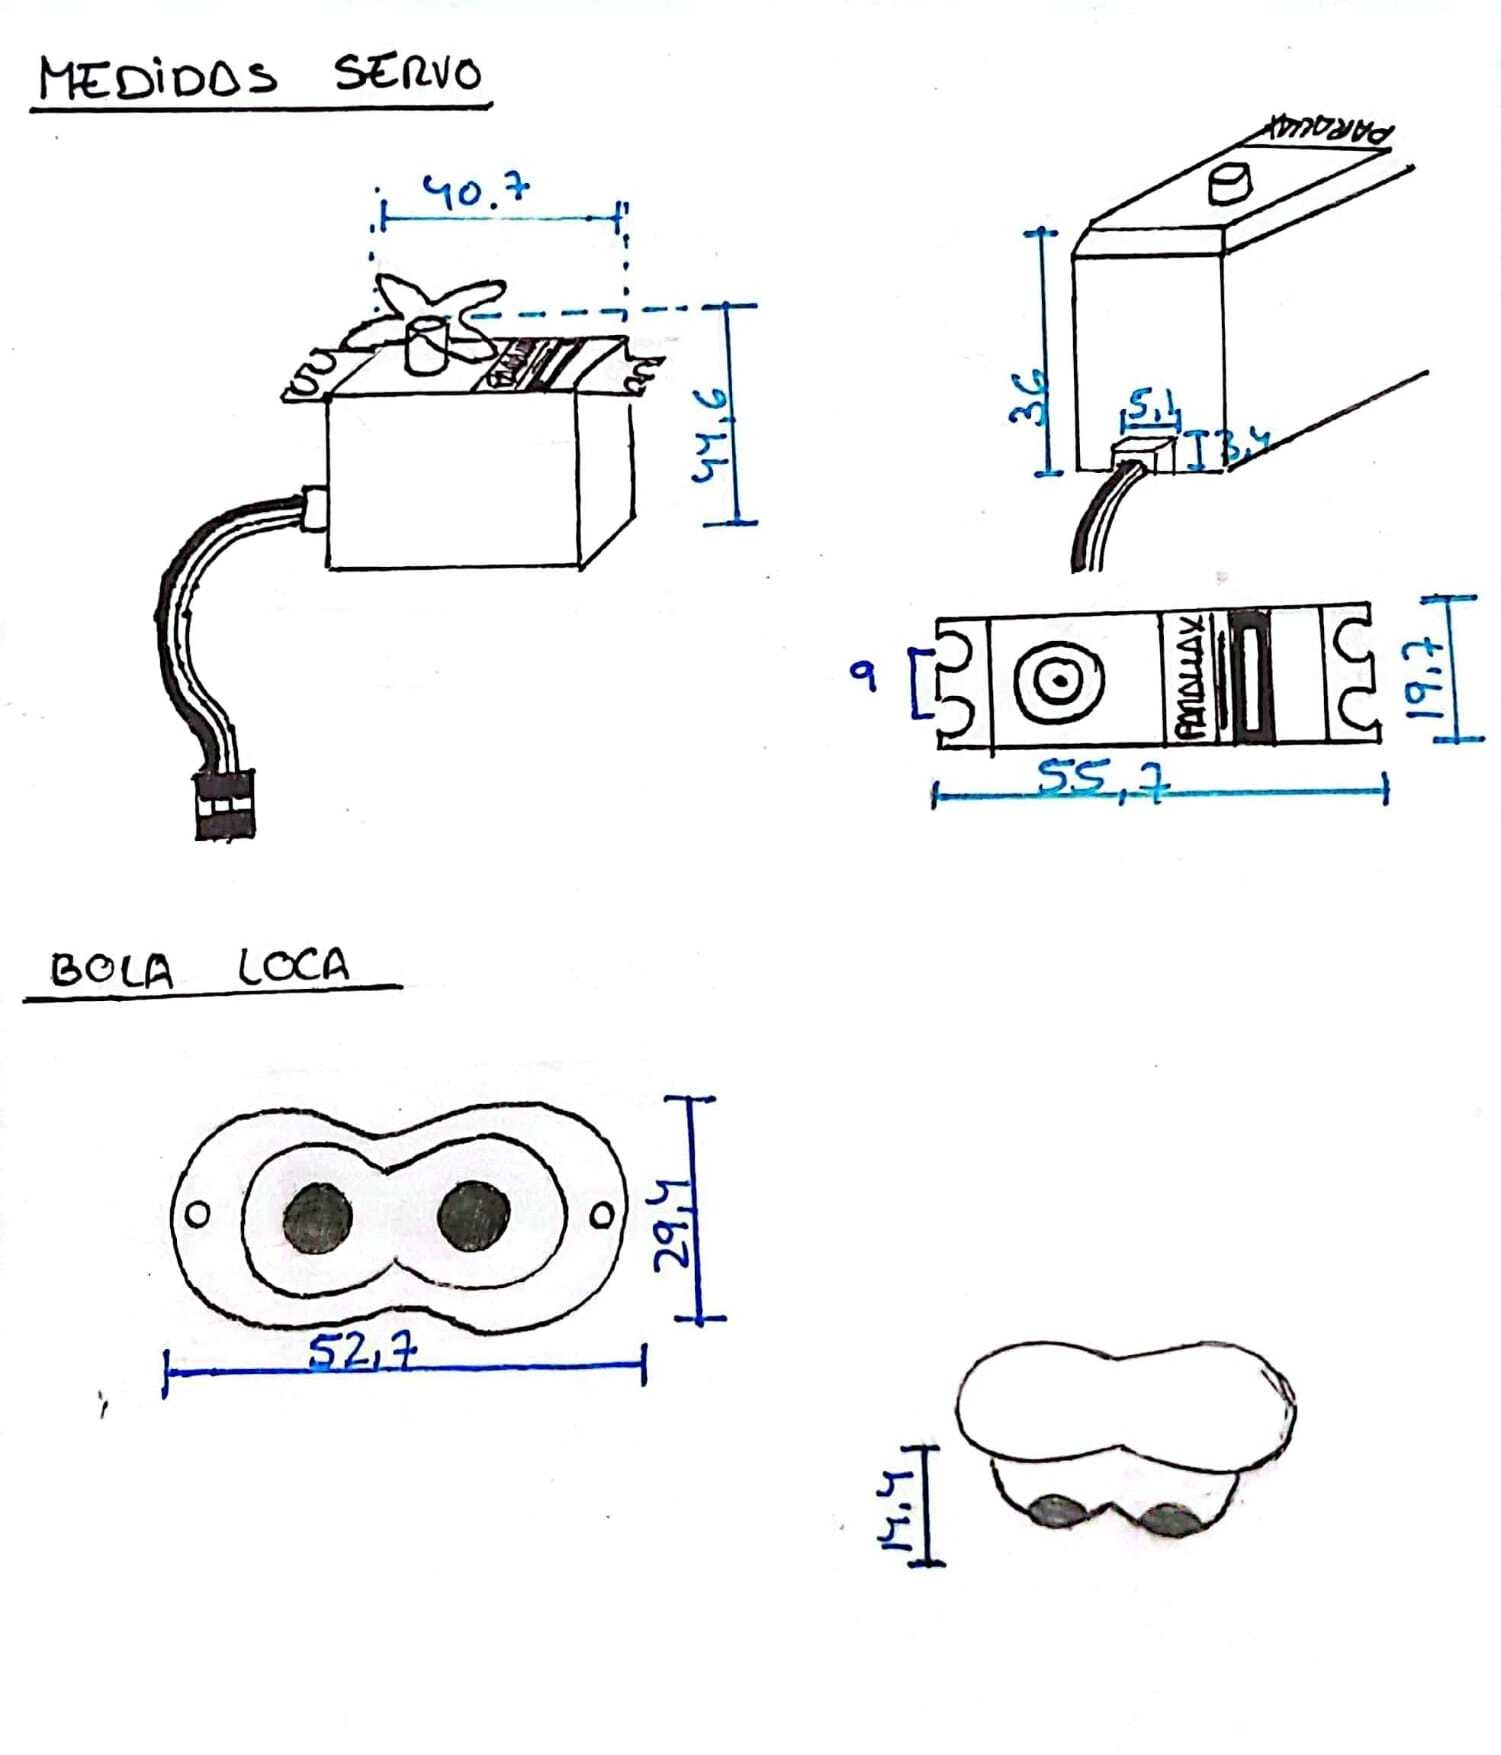
\includegraphics[width=\linewidth]{figs/cap5/planos4.jpeg}
		\caption*{\centering}
	\end{minipage}
	\caption{Planos de los componentes}
	\label{fig:planos}
\end{figure}


\begin{figure}[ht!]
	\centering
	\begin{minipage}{0.4\linewidth}
		\centering
		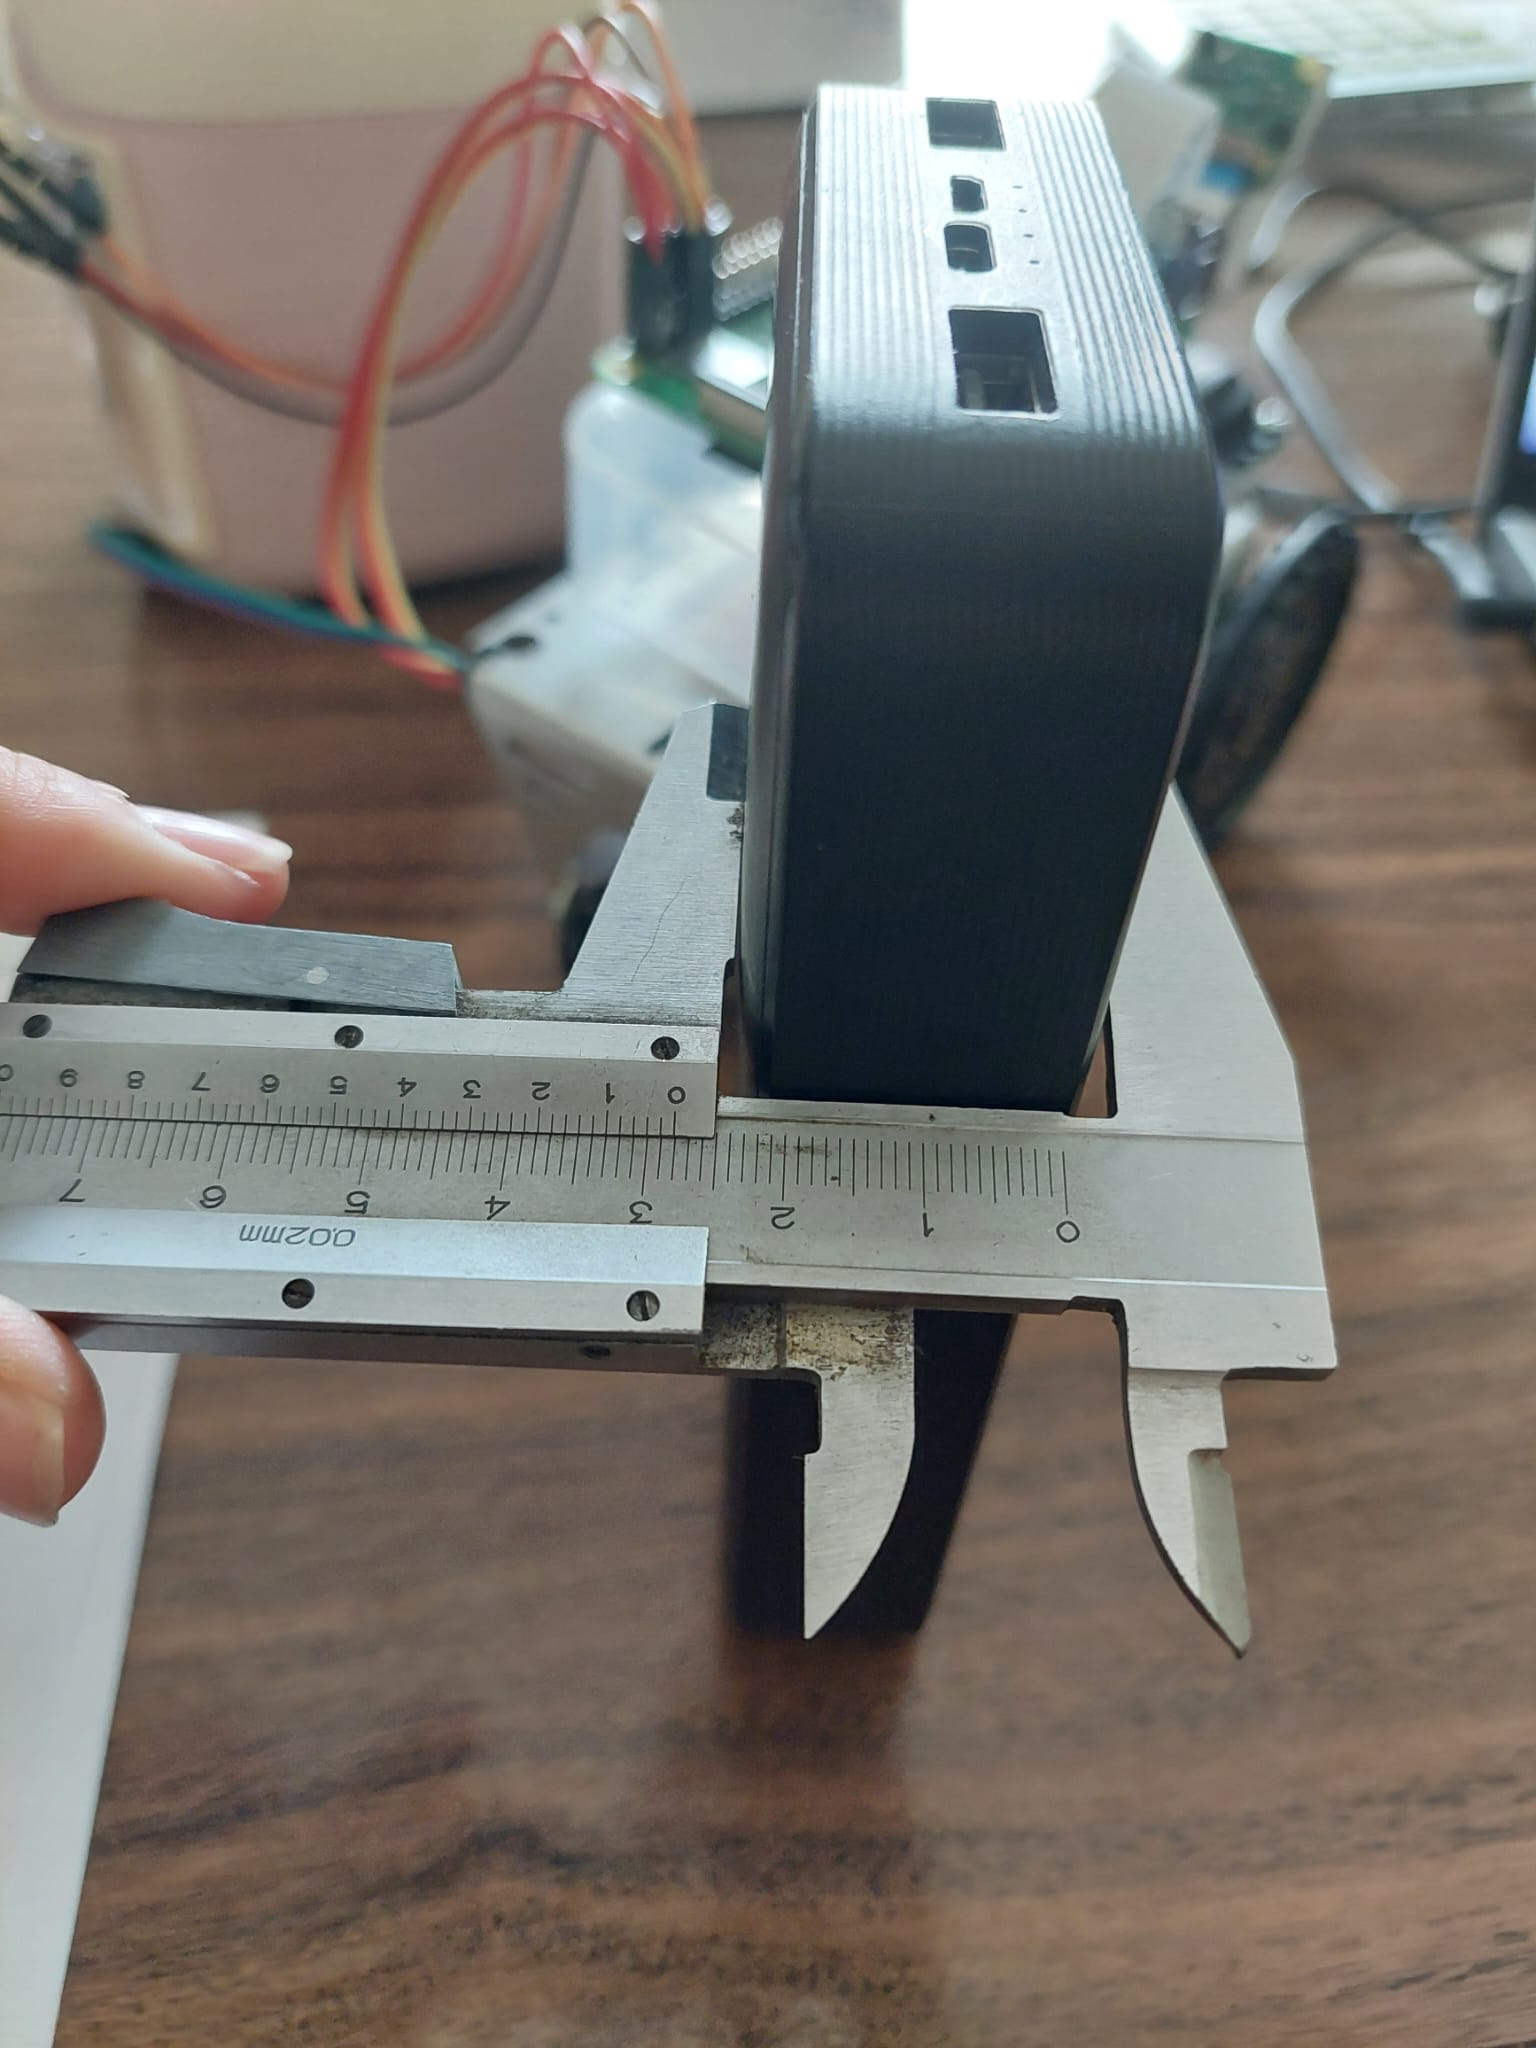
\includegraphics[width=\linewidth]{figs/cap5/calib1.jpeg}
		\caption*{\centering}
	\end{minipage}
	\hspace{2cm}
	\begin{minipage}{0.4\linewidth}
		\centering
		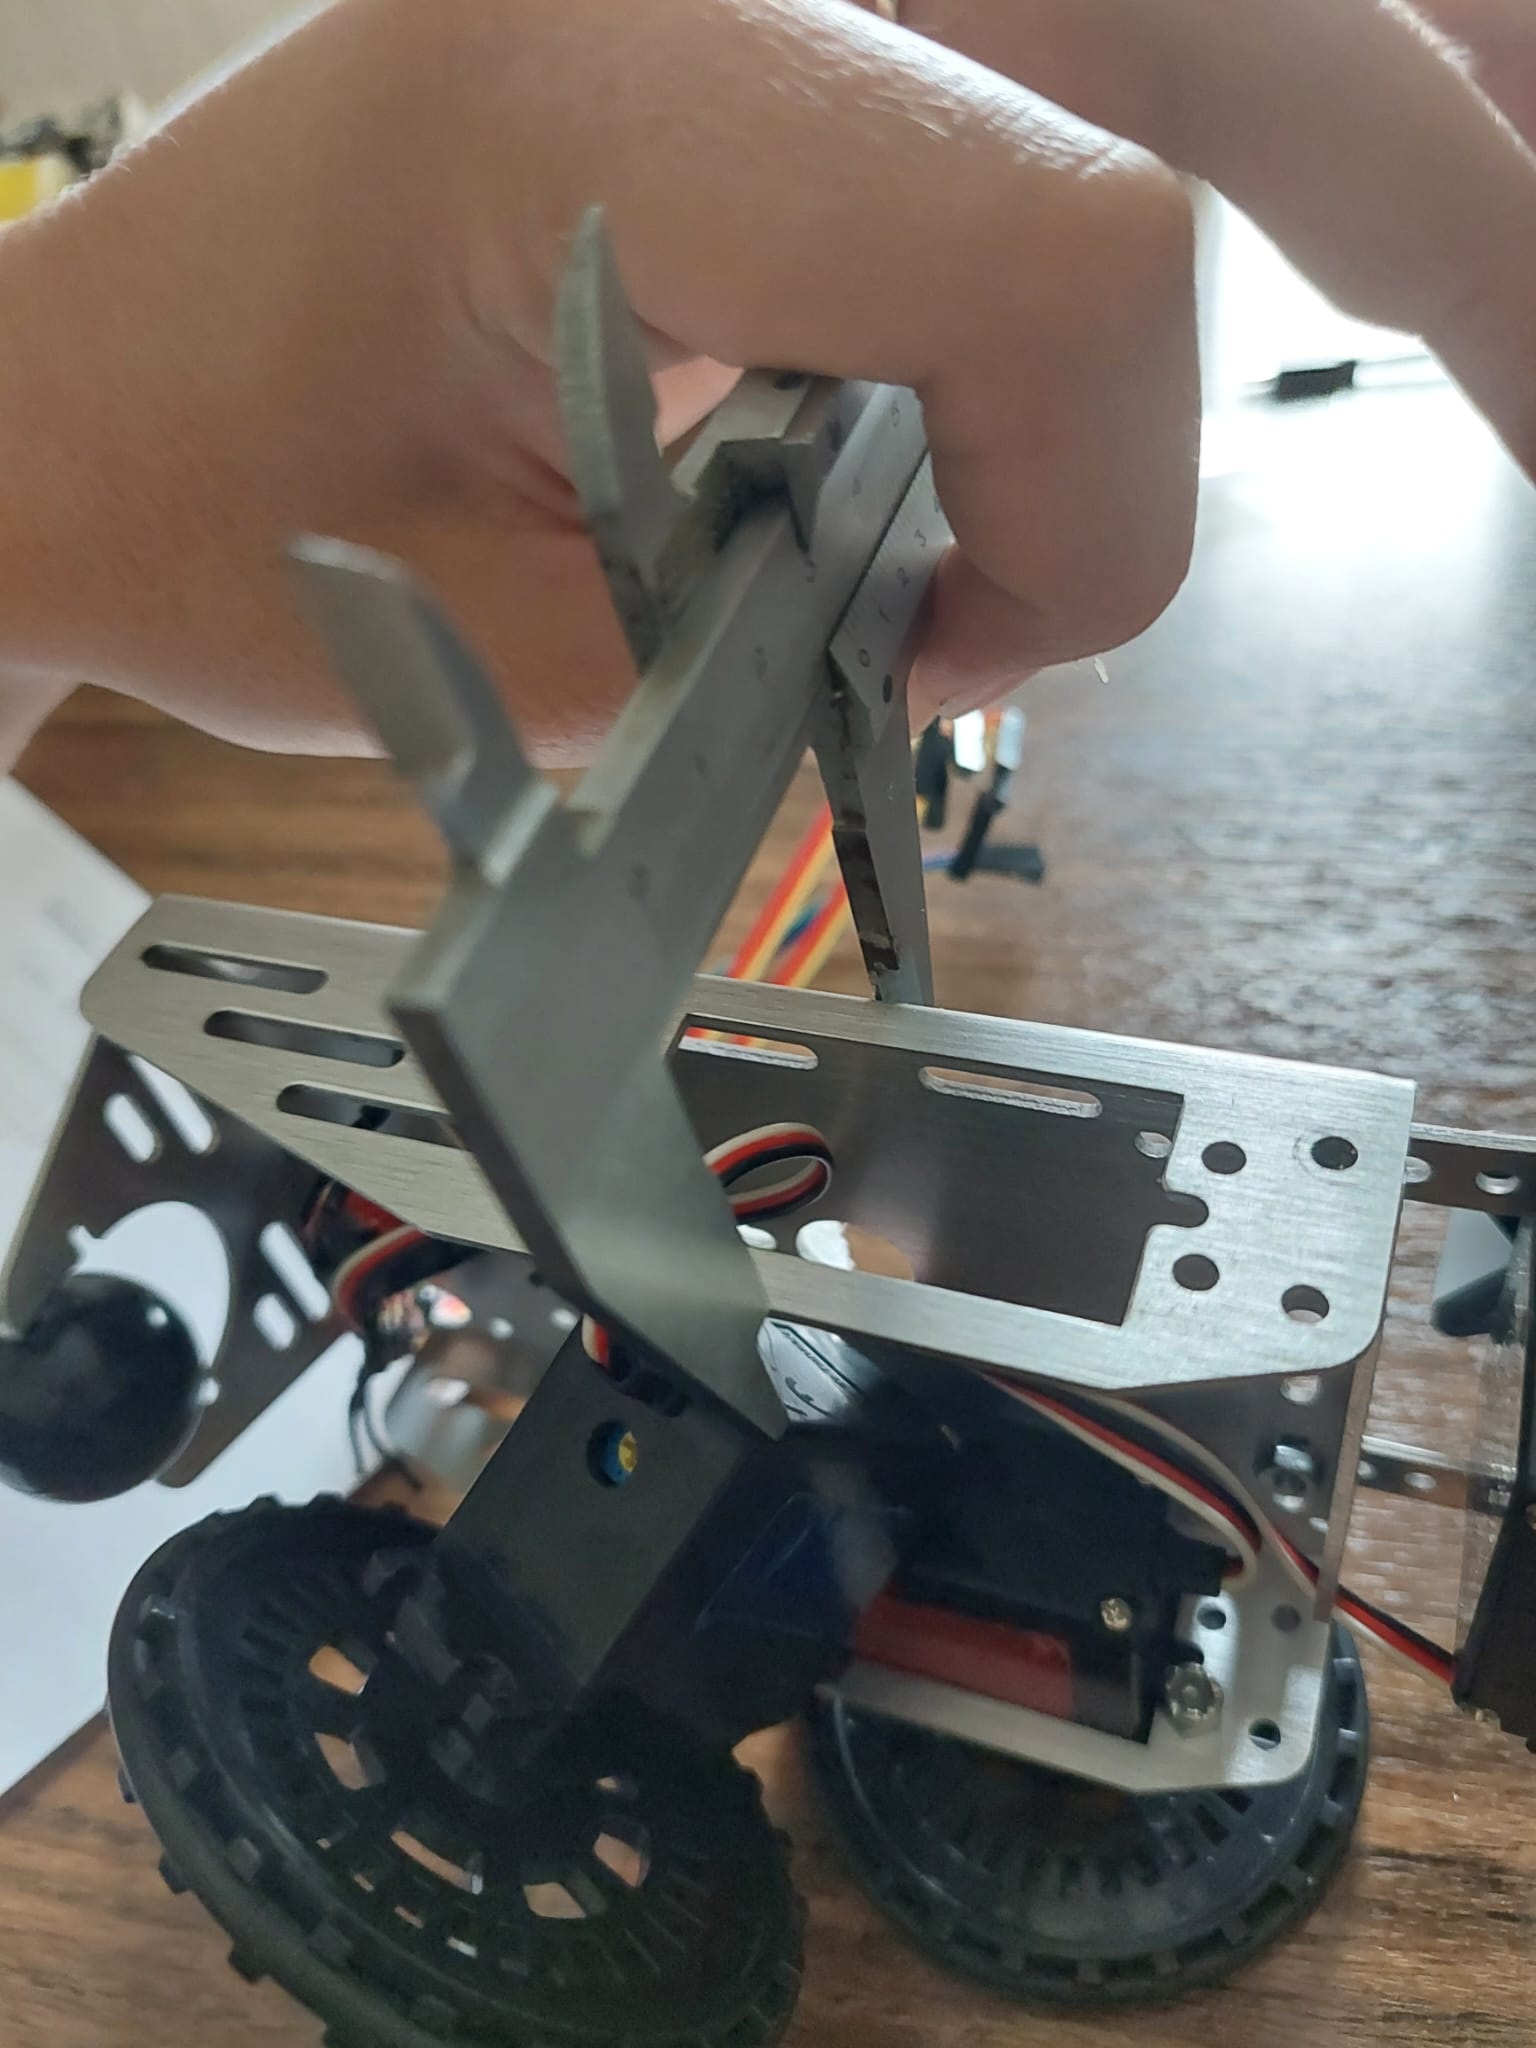
\includegraphics[width=\linewidth]{figs/cap5/calib2.jpeg}
		\caption*{\centering}
	\end{minipage}
	\caption{Usando el calibre}
	\label{fig:calibre}
\end{figure}

\setcounter{footnote}{64}

Para el diseño de este robot, se ha empleado la herramienta de modelado FreeCAD\footnote{\url{https://www.freecad.org/}} con el objetivo de utilizar \textit{software} libre, permitiendo que cualquier persona pueda acceder y modificar las piezas. El diseño se ha dividido en cuatro partes, cada una con una finalidad específica, las cuales se describirán a continuación.

Para llevar a cabo el diseño de todas las piezas, se han seguido los tutoriales de dos cursos de FreeCAD impartidos por Juan González (también conocido como Obijuan)\footnote{\url{https://www.youtube.com/watch?v=2_DbFzFV9D4&list=PLmnz0JqIMEzWQV-3ce9tVB_LFH9a91YHf}}, y el curso de FreeCAD para ingenieros de dcahue-ingeniería\footnote{\url{https://www.youtube.com/watch?v=4zp2DrWv8Wk&list=PLEpca2UUEwQeHp33w36SCzmCz_KKzaMKr&index=11}}, ambos fundamentales en el desarrollo del proyecto.

Además, se han utilizado otros tutoriales específicos, como los dedicados a la creación de \textit{shape binders}\footnote{\url{https://www.youtube.com/watch?v=MCY5IrWrHrU}} y la realización de planos inclinados\footnote{\url{https://www.youtube.com/watch?v=T4hKW1mLrCw}}, esenciales para diseñar la inclinación de la cámara.

\subsection{Pieza base}

La pieza base ha sido diseñada para alojar los motores de las ruedas y de la cámara. En la parte trasera, incorpora un prisma rectangular destinado a la colocación de la rueda loca, mientras que en el lado izquierdo cuenta con un orificio circular para sujetar la \textit{powerbank}. En la parte superior, se han añadido seis aberturas rectangulares para permitir el paso ordenado de los cables, manteniendo una estética limpia y organizada desde el exterior.

Además, dispone de cuatro orificios circulares que permiten fijar la pieza superior mediante tornillos. Se puede encontrar tanto su versión compatible con FreeCAD\footnote{\url{https://github.com/RoboticsURJC/tfg-jlopez/blob/main/design/base.FCStd}} como con el formato de diseño 3D por excelencia, STL\footnote{\url{https://github.com/RoboticsURJC/tfg-jlopez/blob/main/design/base.stl}}. La Figura \ref{fig:pbase} muestra la pieza base desde distintas perspectivas, tal como será preparada para la impresión en una impresora 3D convencional. Por su parte, la Figura \ref{fig:pbasemontada} presenta nuevamente la pieza base, pero esta vez equipada con los componentes de \textit{hardware} necesarios.

\begin{figure}[ht!]
	\centering
	\begin{minipage}{0.45\linewidth}
		\centering
		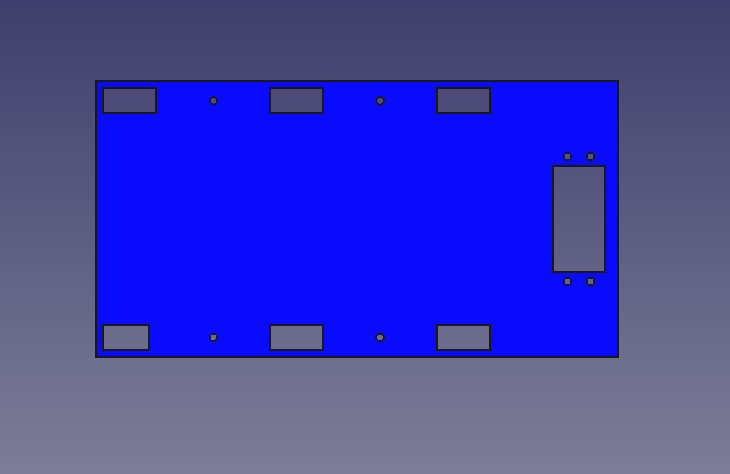
\includegraphics[width=\linewidth]{figs/cap5/basevistasuperiorsin.png}
		\caption*{\centering Vista superior}
	\end{minipage}
	\hspace{1cm}
	\begin{minipage}{0.45\linewidth}
		\centering
		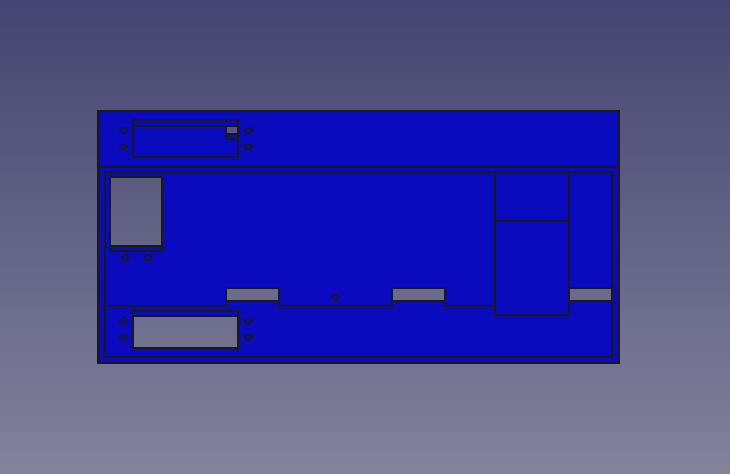
\includegraphics[width=\linewidth]{figs/cap5/basevistaladosin.png}
		\caption*{\centering Vista inferior}
	\end{minipage}
	\hspace{1cm}
	\begin{minipage}{0.45\linewidth}
		\centering
		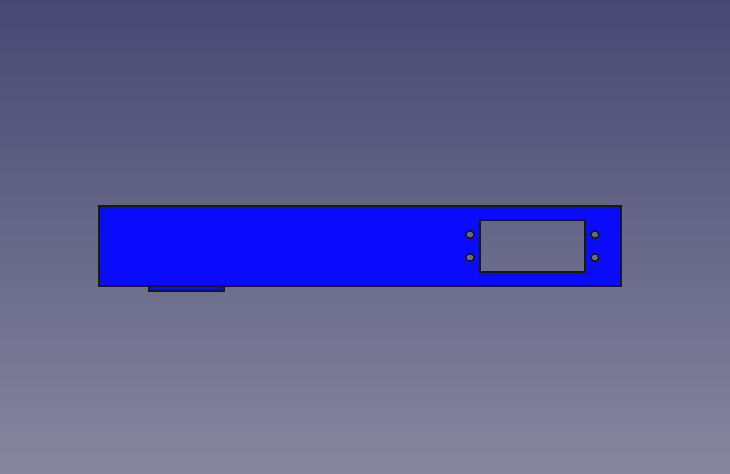
\includegraphics[width=\linewidth]{figs/cap5/basevistalateralsin.png}
		\caption*{\centering Vista lateral}
	\end{minipage}
	\hspace{1cm}
	\begin{minipage}{0.45\linewidth}
		\centering
		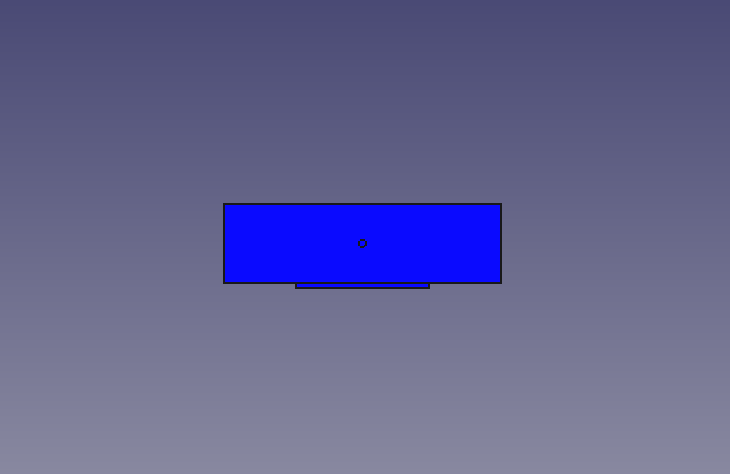
\includegraphics[width=\linewidth]{figs/cap5/basetraserasin.png}
		\caption*{\centering Vista lateral izquierdo}
	\end{minipage}

	\caption{Pieza base}
	\label{fig:pbase}
\end{figure}


\begin{figure}[ht!]
	\centering
	\begin{minipage}{0.45\linewidth}
		\centering
		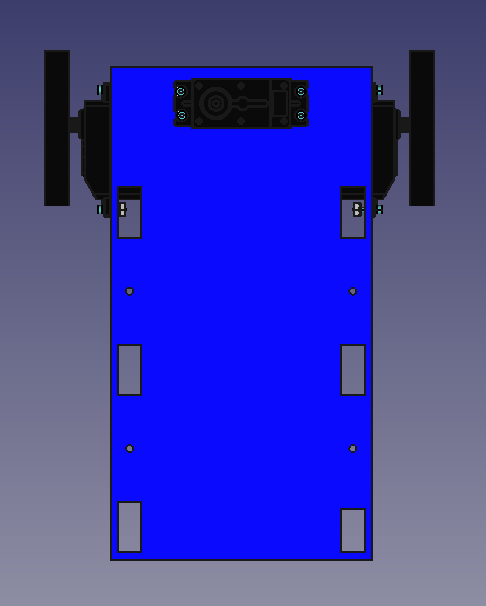
\includegraphics[width=\linewidth]{figs/cap5/basecon1.png}
		\caption*{\centering}
	\end{minipage}
	\hspace{1cm}
	\begin{minipage}{0.45\linewidth}
		\centering
		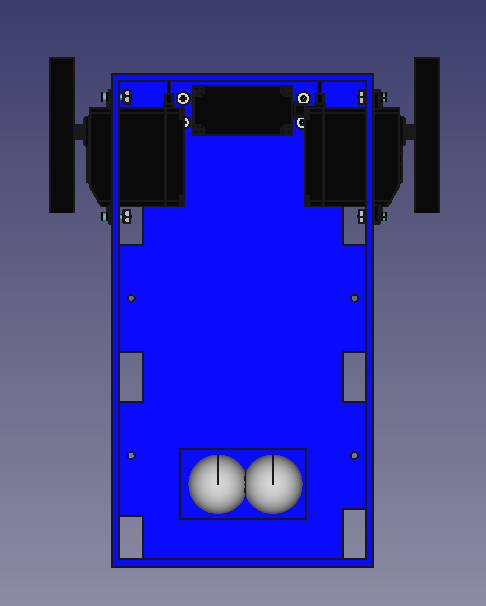
\includegraphics[width=\linewidth]{figs/cap5/basecon2.png}
		\caption*{\centering}
	\end{minipage}
	\caption{Pieza base atornillada}
	\label{fig:pbasemontada}
\end{figure}

\subsection{Pieza cámara}

 
Para posicionar la cámara de manera que mire hacia el suelo y pueda captar los baches, es necesario fijarla con una rotación sobre el eje y. En este caso, dicha rotación es de 50 grados, o 130 grados si se toma como referencia la base de la pieza que va atornillada al motor (Figura \ref{fig:rot}). Esta base cuenta con dos orificios diagonales que permiten su fijación al motor.

\begin{figure} [h!]
	\begin{center}
		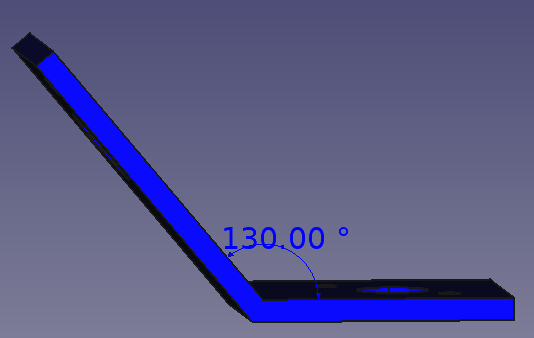
\includegraphics[width=8cm]{figs/cap5/rot.png}
	\end{center}
	\caption{Inclinación de la cámara} 
\label{fig:rot}
\end{figure}

La parte inclinada de la pieza incluye un orificio diseñado para alojar el sensor CMOS, garantizando una correcta alineación y visión. Además, esta sección tiene dos orificios adicionales para asegurar el sensor CMOS y mantenerlo firmemente en su lugar. Se puede encontrar tanto su versión compatible con FreeCAD\footnote{\url{https://github.com/RoboticsURJC/tfg-jlopez/blob/main/design/camara.FCStd}} como con el formato STL\footnote{\url{https://github.com/RoboticsURJC/tfg-jlopez/blob/main/design/camara.stl}}. La Figura \ref{fig:pcamara} muestra la pieza de la cámara desde distintas perspectivas, tal como será preparada para la impresión en una impresora 3D convencional. Por su parte, la Figura \ref{fig:pcamaramontada} presenta nuevamente la pieza de la cámara, pero esta vez atornillada sobre los componentes \textit{hardware} necesarios. 

\begin{figure}[ht!]
	\centering
	\begin{minipage}{0.45\linewidth}
		\centering
		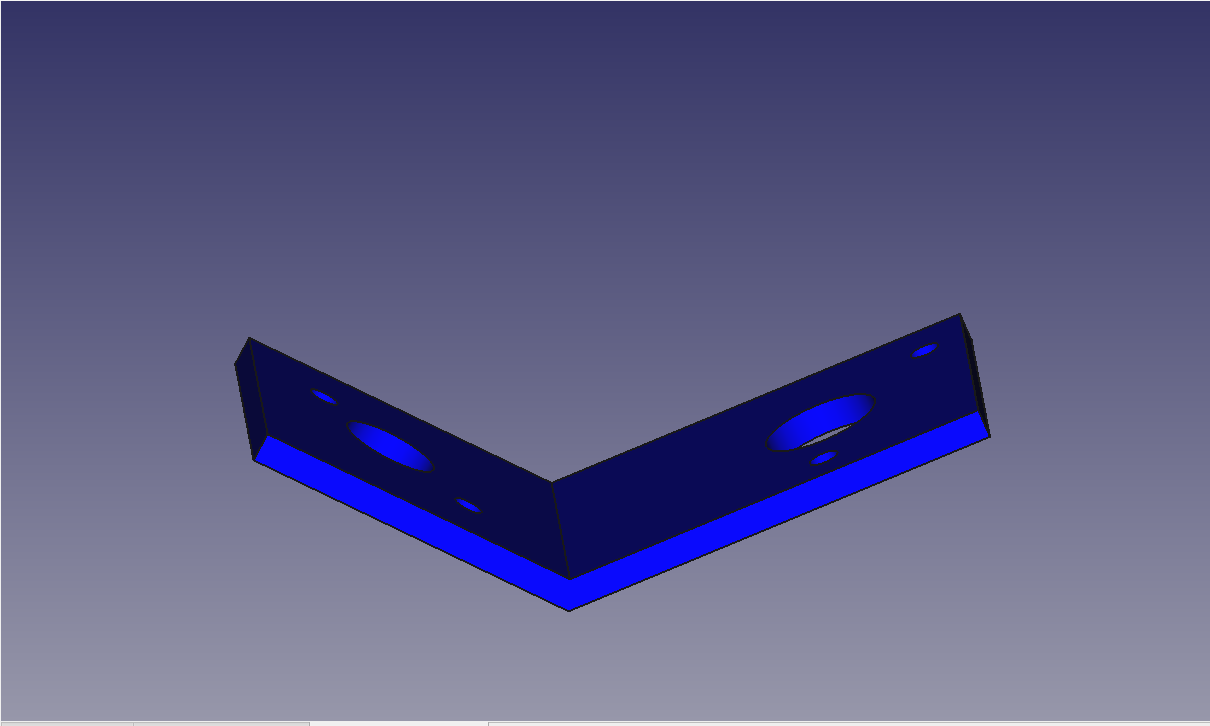
\includegraphics[width=\linewidth]{figs/cap5/camera2sin.png}
		\caption*{\centering}
	\end{minipage}
	\hspace{1cm}
	\begin{minipage}{0.45\linewidth}
		\centering
		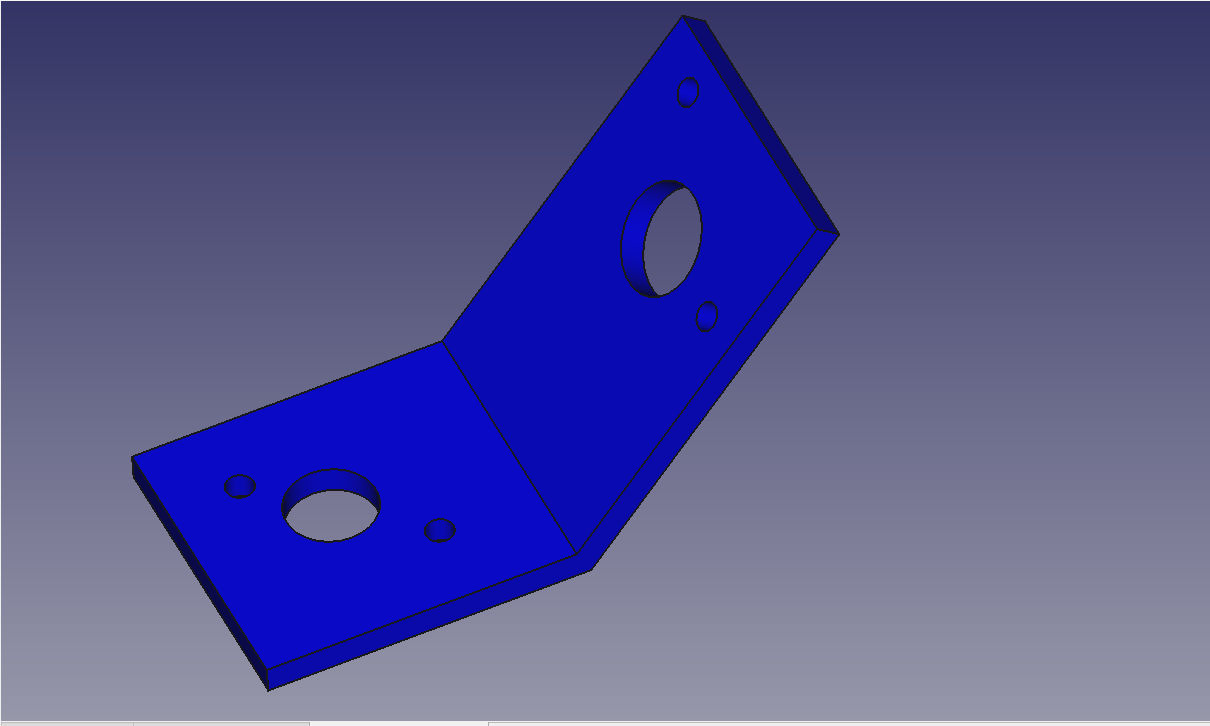
\includegraphics[width=\linewidth]{figs/cap5/camera3sin.png}
		\caption*{\centering}
	\end{minipage}
	
	\caption{Pieza cámara}
	\label{fig:pcamara}
\end{figure}


\begin{figure}[ht!]
	\centering
	\begin{minipage}{0.45\linewidth}
		\centering
		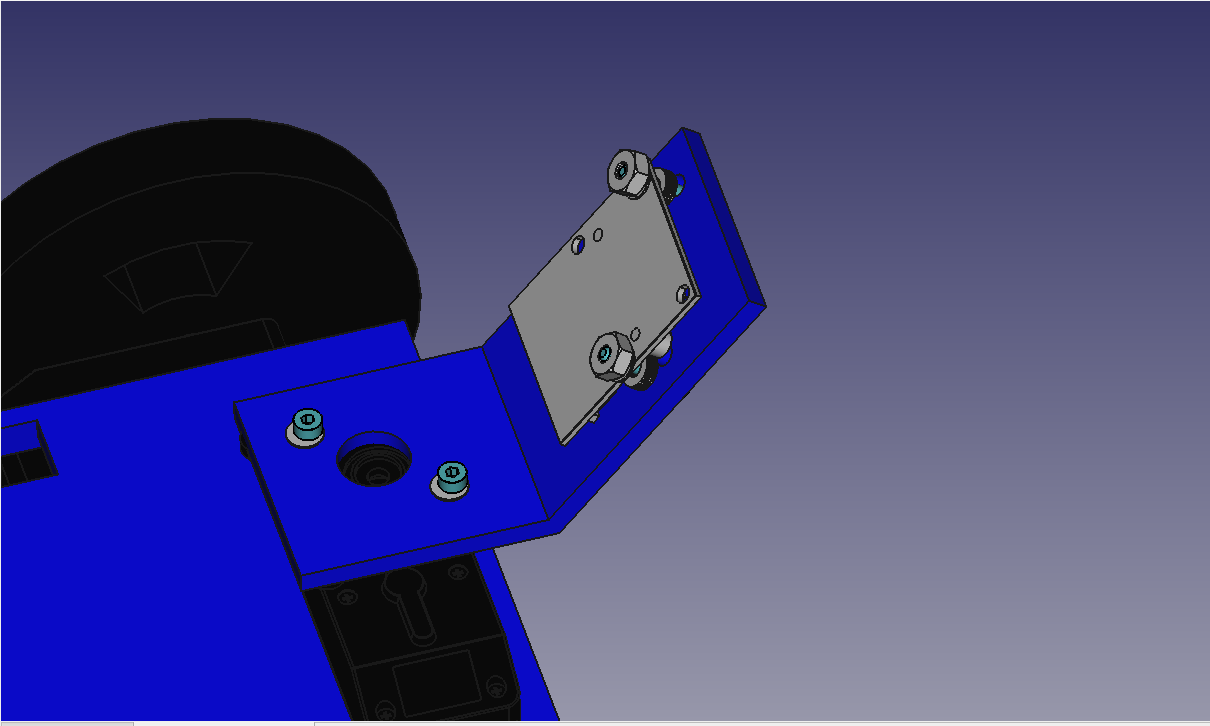
\includegraphics[width=\linewidth]{figs/cap5/camera2con.png}
		\caption*{\centering}
	\end{minipage}
	\hspace{1cm}
	\begin{minipage}{0.45\linewidth}
		\centering
		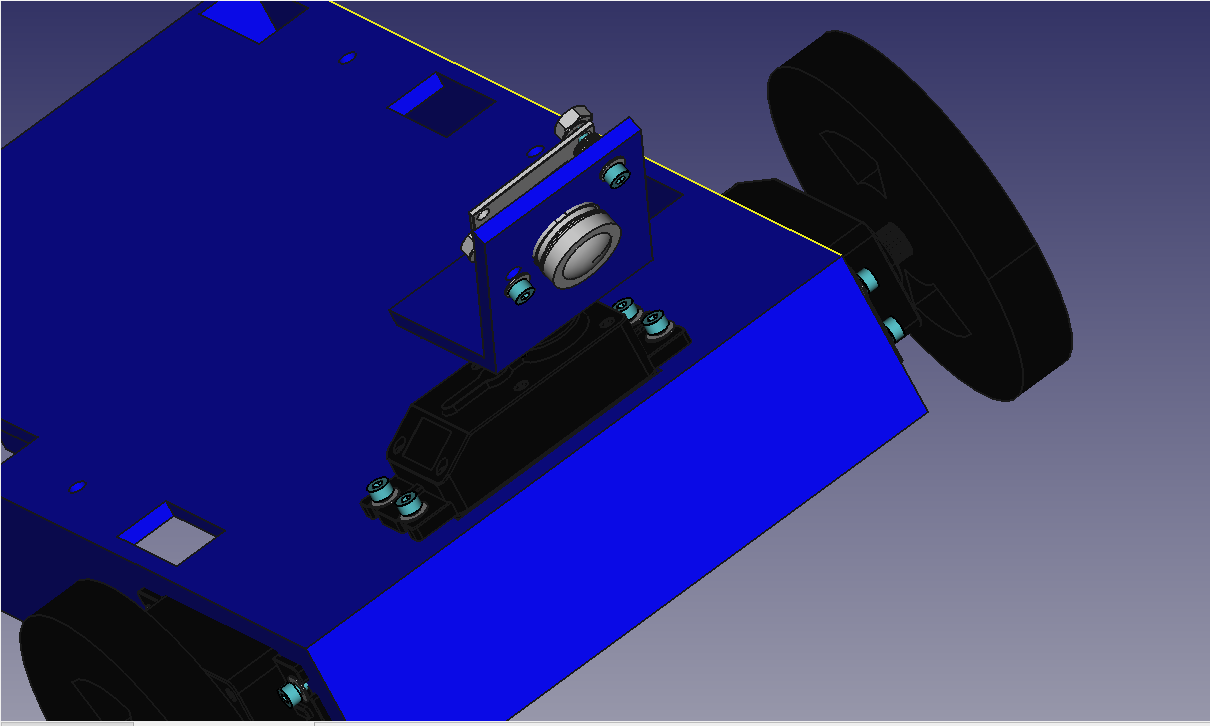
\includegraphics[width=\linewidth]{figs/cap5/camera3con.png}
		\caption*{\centering}
	\end{minipage}
	\caption{Pieza cámara atornillada}
	\label{fig:pcamaramontada}
\end{figure}


\subsection{Pieza superior}


Esta pieza superior ha sido diseñada para alojar la placa Raspberry Pi, el módulo GPS y la \textit{powerbank} en su interior. En la cara superior se encuentran doce orificios circulares destinados a atornillar tanto la Raspberry Pi como el módulo GPS. Además, en esta misma cara hay seis aberturas que se conectan con la cara inferior, alineándose con las aberturas correspondientes de la pieza base para garantizar un paso de cables ordenado.

La cara inferior, además de las seis aberturas, incluye cuatro orificios adicionales para permitir el atornillado de la pieza base. En el lateral izquierdo, la pieza está abierta para facilitar la inserción de la \textit{powerbank}, mientras que en el lado derecho cuenta con dos cuadrantes que permiten retirar la \textit{powerbank} cuando sea necesario. Esta pieza está disponible tanto en formato compatible con FreeCAD como en STL.

La Figura \ref{fig:psuperior} muestra la pieza base desde varias perspectivas, lista para la impresión en una impresora 3D convencional. La Figura \ref{fig:psuperiormontada} presenta nuevamente la pieza base, pero equipada con los componentes de hardware necesarios.


\begin{figure}[ht!]
	\centering
	\begin{minipage}{0.45\linewidth}
		\centering
		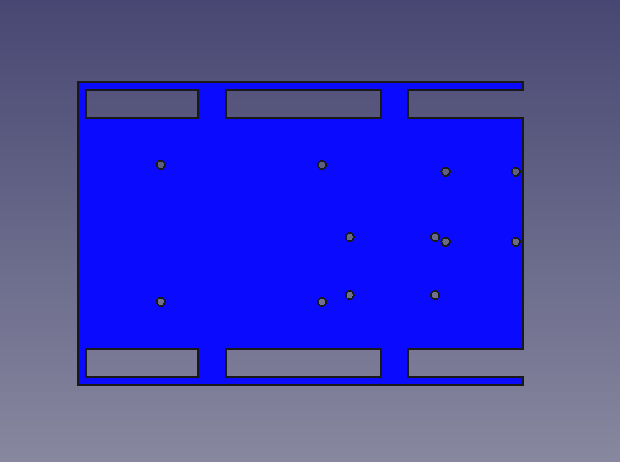
\includegraphics[width=\linewidth]{figs/cap5/superior1.png}
		\caption*{\centering Vista superior}
	\end{minipage}
	\hspace{1cm}
	\begin{minipage}{0.45\linewidth}
		\centering
		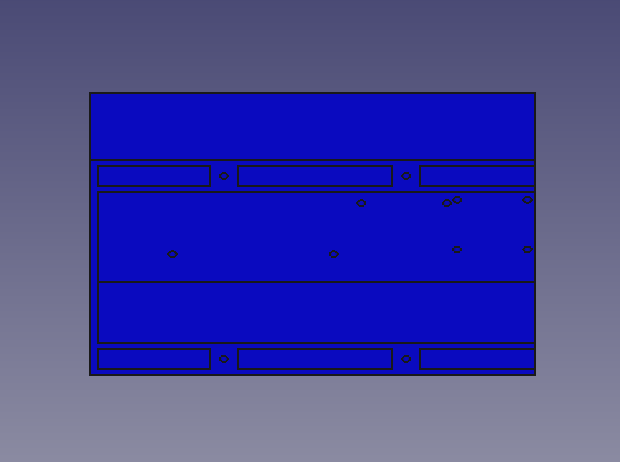
\includegraphics[width=\linewidth]{figs/cap5/superior2.png}
		\caption*{\centering Vista inferior}
	\end{minipage}
	\hspace{1cm}
	\begin{minipage}{0.45\linewidth}
		\centering
		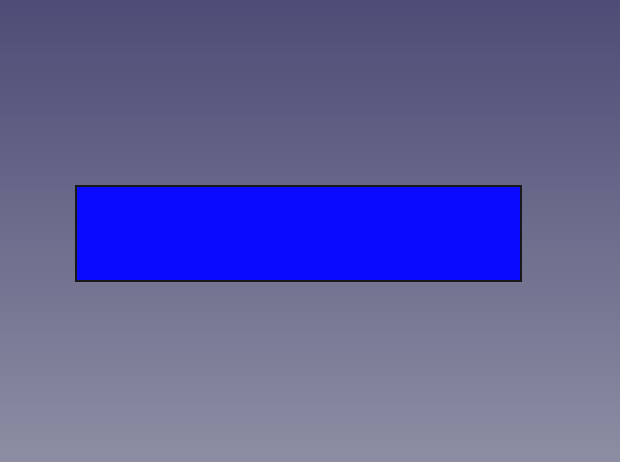
\includegraphics[width=\linewidth]{figs/cap5/superior3.png}
		\caption*{\centering Vista lateral}
	\end{minipage}
	\hspace{1cm}
	\begin{minipage}{0.45\linewidth}
		\centering
		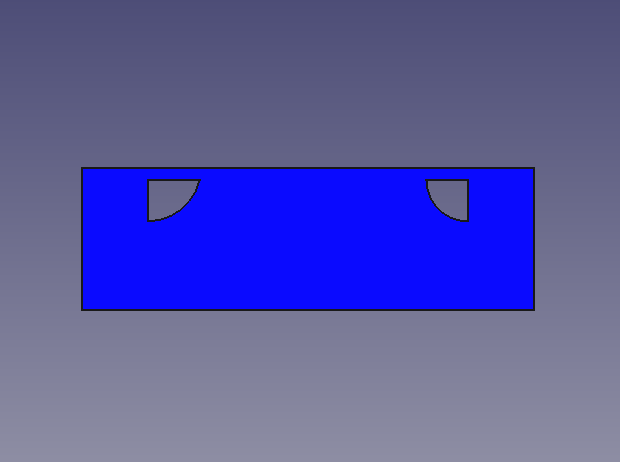
\includegraphics[width=\linewidth]{figs/cap5/superior4.png}
		\caption*{\centering Vista lateral izquierdo}
	\end{minipage}
	
	\caption{Pieza superior}
	\label{fig:psuperior}
\end{figure}


\begin{figure}[ht!]
	\centering
	\begin{minipage}{0.45\linewidth}
		\centering
		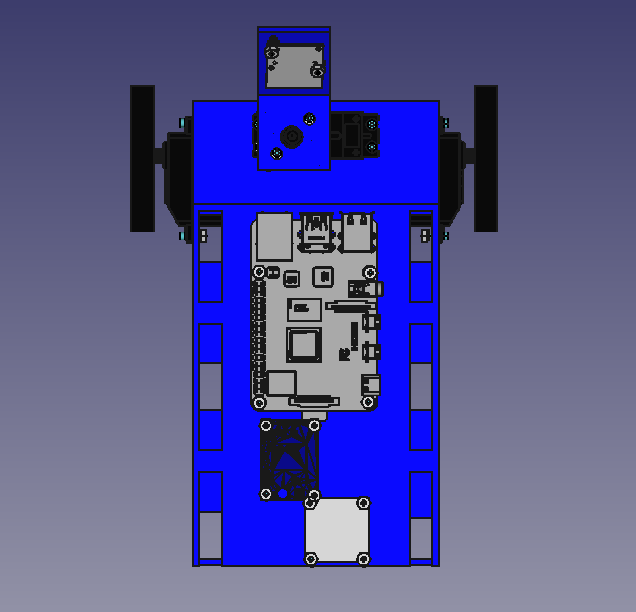
\includegraphics[width=\linewidth]{figs/cap5/superior1m.png}
		\caption*{\centering}
	\end{minipage}
	\hspace{1cm}
	\begin{minipage}{0.45\linewidth}
		\centering
		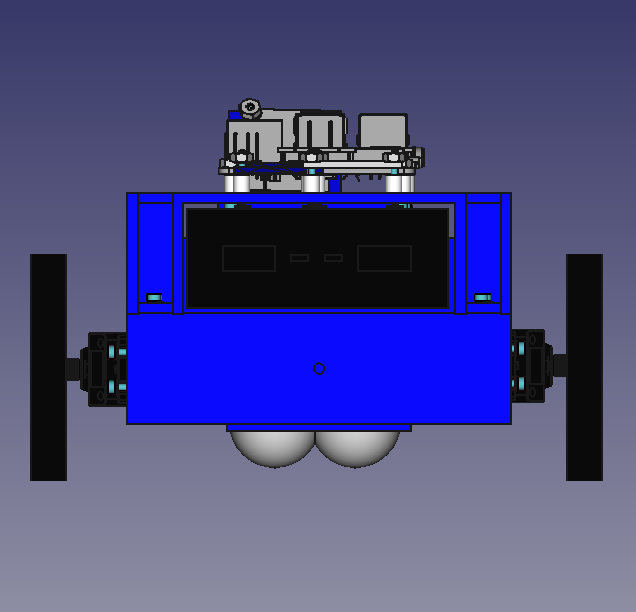
\includegraphics[width=\linewidth]{figs/cap5/superior2m.png}
		\caption*{\centering}
	\end{minipage}
	\caption{Pieza superior atornillada}
	\label{fig:psuperiormontada}
\end{figure}


\subsection{Pieza sujección trasera}

Para asegurar que la \textit{powerbank} se mantenga en su lugar dentro del robot, se ha diseñado una pieza que se atornilla en el lado izquierdo de la base. Esta pieza es un prisma rectangular con más de 30 mm de altura, aproximadamente 5 mm de largo y 3 mm de ancho (Figura \ref{fig:ptrasera}). Su función es mantener la \textit{powerbank} en su hueco. La pieza debe colocarse en posición vertical para evitar que la \textit{powerbank} se deslice, y en posición horizontal cuando se desee retirarla. Existe una versión en FreeCAD\footnote{\url{https://github.com/RoboticsURJC/tfg-jlopez/blob/main/design/sujeccion-trasera.FCStd}} y otra en formato STL\footnote{\url{https://github.com/RoboticsURJC/tfg-jlopez/blob/main/design/sujeccion-trasera.stl}}. La Figura \ref{fig:traseracon} muesta cómo quedaría montada la pieza sobre el robot.

\begin{figure}[ht!]
	\centering
	\begin{minipage}{0.45\linewidth}
		\centering
		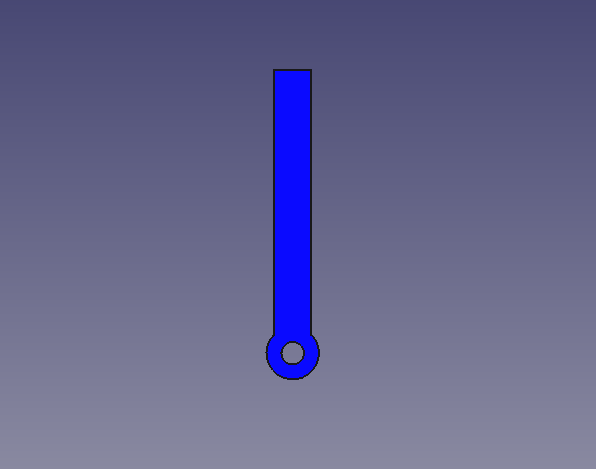
\includegraphics[width=\linewidth]{figs/cap5/trasera1.png}
		\caption*{\centering}
	\end{minipage}
	\hspace{1cm}
	\begin{minipage}{0.45\linewidth}
		\centering
		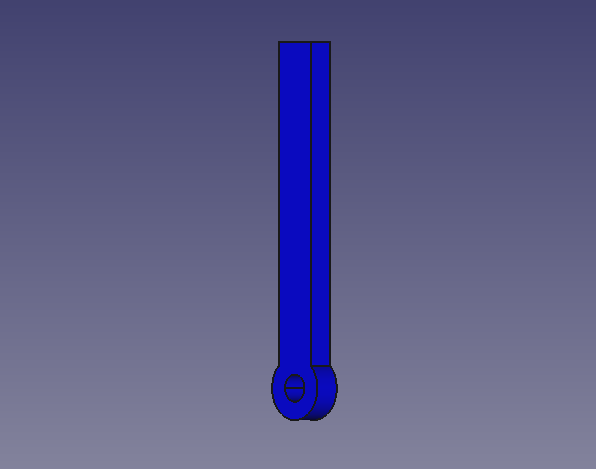
\includegraphics[width=\linewidth]{figs/cap5/trasera2.png}
		\caption*{\centering}
	\end{minipage}
	\caption{Pieza sujección trasera}
	\label{fig:ptrasera}
\end{figure}


\begin{figure} [h!]
	\begin{center}
		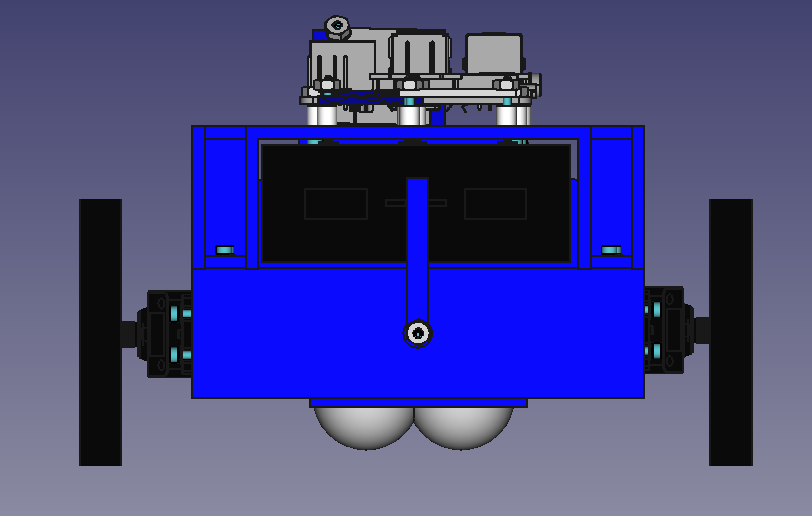
\includegraphics[width=8cm]{figs/cap5/traseracon.png}
	\end{center}
	\caption{Pieza sujección trasera montada} 
	\label{fig:traseracon}
\end{figure}

\section{Impresión y montaje}


Dificultades imprimiendo: con la impresora del instituto. Incluir características de la impresora y de la impresión usada.

Impresión de Gonzalo
Características: 

Impresora FDM Creality Ender3 V2
Slicer Software: UltiMaker Cura

QUALITY:
Layer height: 0.2 mm
Line width: 0.4 mm

WALLS: 
Wall thickness: 0.8 mm
Wall line count: 2
Z sean alignment: "Sharpest corner"
Seam corner preference: "Smart hiding"

INFILL:
Infill density: 15%
Infill pattern: "Gyroid"

SPEED:
Print speed: 50 mm/s
Initial layer speed: 20 mm/s


Incluir una lista de los tornillos usados, hama  beads...\\\\



Incluir imagen completa que incluya el Google Coral USB\\\\\\


INCLUIR MUCHAS FOTOS\\\\\\



CApítulo 6: incluir lo de openvision paper\\
capitulo 7: explicar experimentos impresora \\

\section{Snippets}

Puede resultar interesante, para clarificar la descripción, mostrar fragmentos de código (o \textit{snippets}) ilustrativos. En el Código \ref{cod:codejemplo} vemos un ejemplo escrito en \texttt{C++}.

\begin{code}[h]
\begin{lstlisting}[language=C++]
void Memory::hypothesizeParallelograms () {
  for(it1 = this->controller->segmentMemory.begin(); it1++) {
    squareFound = false; it2 = it1; it2++;
    while ((it2 != this->controller->segmentMemory.end()) && (!squareFound)) {
      if (geometry::haveACommonVertex((*it1),(*it2),&square)) {
        dist1 = geometry::distanceBetweenPoints3D ((*it1).start, (*it1).end);
        dist2 = geometry::distanceBetweenPoints3D ((*it2).start, (*it2).end);
      }
    // [...]
\end{lstlisting}
\caption[Función para buscar elementos 3D en la imagen]{Función para buscar elementos 3D en la imagen}
\label{cod:codejemplo}
\end{code}

En el Código \ref{cod:codejemplo2} vemos un ejemplo escrito en \texttt{Python}.

\begin{code}[h]
\begin{lstlisting}[language=Python]
def mostrarValores():
    print (w1.get(), w2.get())

master = Tk()
w1 = Scale(master, from_=0, to=42)
w1.pack()
w2 = Scale(master, from_=0, to=200, orient=HORIZONTAL)
w2.pack()
Button(master, text='Show', command=mostrarValores).pack()

mainloop()
\end{lstlisting}
\caption[Cómo usar un Slider]{Cómo usar un Slider}
\label{cod:codejemplo2}
\end{code}

\section{Verbatim}

Para mencionar identificadores usados en el código ---como nombres de funciones o variables--- en el texto, usa el entorno literal o verbatim \verb|hypothesizeParallelograms()|. También se puede usar este entorno para varias líneas, como se ve a continuación:

\begin{verbatim}
void Memory::hypothesizeParallelograms () {
  // add your code here
}
\end{verbatim}

\section{Ecuaciones}

Si necesitas insertar alguna ecuación, puedes hacerlo. Al igual que las figuras, no te olvides de referenciarlas. A continuación se exponen algunas ecuaciones de ejemplo: Ecuación \ref{ec:ec1} y Ecuación \ref{ec:ec2}.

\begin{myequation}[h]
\begin{equation}
H = 1 - \frac{\sum_{i=0}^{N}\frac{(\frac{d_{j_s} + d_{j_e}}{2})}{N}}{M}
\nonumber
\label{ec:ec1}
\end{equation}
\caption[Ejemplo de ecuación con fracciones]{Ejemplo de ecuación con fracciones}
\end{myequation} 

\begin{myequation}[h]
\begin{equation}
v(entrada)= \left\{
	\begin{array}{lcc}
		0 & \mbox{if} & \epsilon_t < 0.1\\
		K_p\cdot{(T_{t}-T)} & \mbox{if}& 0.1 \leq \epsilon_t < M_t\\
		K_p \cdot M_t & \mbox{if}& M_t < \epsilon_t
	\end{array}
\right.
\label{ec:ec2}
\end{equation}
\caption[Ejemplo de ecuación con array y letras y símbolos especiales]{Ejemplo de ecuación con array y letras y símbolos especiales}
\end{myequation}

\section{Tablas o cuadros}

Si necesitas insertar una tabla, hazlo dígnamente usando las propias tablas de \LaTeX, no usando pantallazos e insertándolas como figuras... En el Cuadro \ref{cuadro:ejemplo} vemos un ejemplo.

\begin{table}[H]
\begin{center}
\begin{tabular}{|c|c|}
\hline
\textbf{Parámetros} & \textbf{Valores} \\
\hline
Tipo de sensor & Sony IMX219PQ[7] CMOS 8-Mpx \\
Tamaño del sensor & 3.674 x 2.760 mm (1/4" format) \\
Número de pixels & 3280 x 2464 (active pixels) \\
Tamaño de pixel & 1.12 x 1.12 um \\
Lente & f=3.04 mm, f/2.0 \\
Ángulo de visión & 62.2 x 48.8 degrees \\
Lente SLR equivalente & 29 mm \\
\hline
\end{tabular}
\caption{Parámetros intrínsecos de la cámara}
\label{cuadro:ejemplo}
\end{center}
\end{table}

En los textos puedes poner palabras en \textit{cursiva}, para aquellas expresiones en sentido \textit{figurado}, palabras como \textit{robota}, que está fuera del diccionario castellano, o bien para resaltar palabras de una colección: \textit{(a)} es la primera letra del abecedario, \textit{(b)} es la segunda, etc.\\

Al poner las dos líneas del anterior párrafo, este aparecerá separado del anterior. Si no las pongo, los párrafos aparecerán pegados. Sigue el criterio que consideres más oportuno.

\section{Segunda sección}
\label{sec:segundaseccion}

No olvides incluir imágenes y referenciarlas, como la Figura \ref{fig:roomba}.

\begin{figure} [h!]
	\begin{center}
		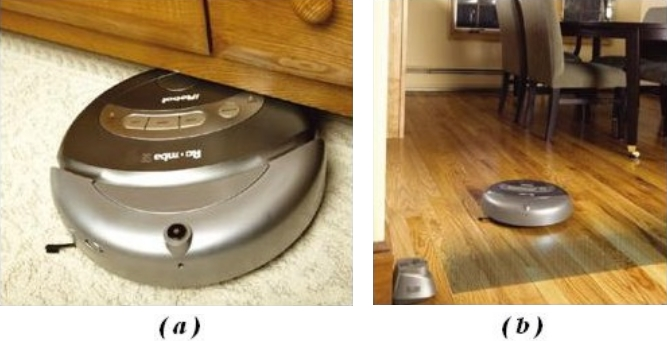
\includegraphics[width=8cm]{figs/roomba}
	\end{center}
	\caption{Robot aspirador Roomba de iRobot.}
	\label{fig:roomba}
\end{figure}\

Ni tampoco olvides de poner las URLs como notas al pie. Por ejemplo, si hablo de la Robocup\footnote{\url{http://www.robocup.org}}.

\subsection{Números}
\label{sec:subseccion}

En lugar de tener secciones interminables, como la Sección \ref{sec:robotica}, divídelas en subsecciones.

Para hablar de números, mételos en el entorno \textit{math} de \LaTeX, por ejemplo, $1.5Kg$. También puedes usar el símbolo del Euro como aquí: 1.500\euro.

\subsection{Listas}

Cuando describas una colección, usa \texttt{itemize} para ítems o \texttt{enumerate} para enumerados. Por ejemplo:

\begin{itemize}
	\item \textit{Entorno de simulación.} Hemos usado dos entornos de simulación: uno en 3D y otro en 2D.
	\item \textit{Entornos reales.} Dentro del campus, hemos realizado experimentos en Biblioteca y en el edificio de Gestión.
\end{itemize}\

\begin{enumerate}
	\item Primer elemento de la colección.
	\item Segundo elemento de la colección.
\end{enumerate}\

\paragraph{Referencias bibliográficas}
\label{sec:referencias}

Cita, sobre todo en este capítulo, referencias bibliográficas que respalden tu argumento. Para citarlas basta con poner la instrucción \verb|\cite| con el identificador de la cita. Por ejemplo: libros como \cite{vega12e}, artículos como \cite{vega19b}, URLs como \cite{vega19a}, tesis como \cite{vega18b}, congresos como \cite{vega18a}, u otros trabajos fin de grado como \cite{vega08b}.

Las referencias, con todo su contenido, están recogidas en el fichero \texttt{bibliografia.bib}. El contenido de estas referencias está en formato \texttt{BibTex}. Este formato se puede obtener en muchas ocasiones directamente, desde plataformas como \texttt{Google Scholar} u otros repositorios de recursos científicos.

Existen numerosos estilos para reflejar una referencia bibliográfica. El estilo establecido por defecto en este documento es APA, que es uno de los estilos más comunes, pero lo puedes modificar en el archivo \texttt{memoria.tex}; concretamente, cambiando el campo \verb|apalike| a otro en la instrucción \verb|\bibliographystyle{apalike}|. 

\

\

\

Y, para terminar este capítulo, resume brevemente qué vas a contar en los siguientes.
